\documentclass{article}
\usepackage{amsmath,amssymb}
\usepackage{graphicx,color}
\usepackage{psfrag}
\usepackage{listings}
\usepackage{color}
\usepackage{url}
%\graphicspath{{/Users/kjiersten/Documents/images/}}

\textwidth=6.5in
\textheight=9.0in
\evensidemargin -0.04cm
\oddsidemargin -0.04cm
\topmargin -0.5in

\newenvironment{choice}{\left\{ \begin{array}{ll}}{\end{array}\right.}

\title{Computational Models of Material Interfaces for the Study of ESWT}

\author{Kirsten Fagnan \thanks{Lawrence Berkeley National Laboratory, 1 Cyclotron Road, Berkeley, 
CA 94720} \and Randall J. LeVeque \thanks{Department of Applied Mathematics, University of 
Washington, Box 352420, Seattle, WA 98195} \and Thomas J. Matula \thanks{Applied Physics 
Laboratory, University of Washington, Seattle, WA 98195}}

\begin{document}

\maketitle

\begin{abstract}
Extracorporeal Shock Wave Therapy (ESWT) is a noninvasive treatment
used to treat a variety of musculoskeletal ailments.
A shock wave is generated in water
and then focused using an acoustic lens or reflector so the energy of
the wave is concentrated in a small treatment region where mechanical stimulation
enhancing healing.
In this work we have computationally
investigated shock wave propagation in ESWT by solving a Lagrangian
form of the isentropic Euler equations in the fluid and linear
elasticity in the bone using high-resolution finite volume methods.
We solve a full three-dimensional system of equations and use adaptive mesh
refinement to concentrate grid cells near the propagating shock.  
We can model complex bone
geometries, the reflection and mode conversion at interfaces, and the
the propagation of the resulting
shear stresses generated within the bone.   We discuss the validity of our
simplified model and present results validating this approach. 
\end{abstract}

\pagestyle{myheadings}
\thispagestyle{plain}



\section{Introduction}
Extracorporeal shock wave therapy (ESWT) is a noninvasive treatment
used to treat musculoskeletal conditions such as bone fractures
that fail to heal (non-unions), necrotic wounds, and strained
tendons.  In this treatment a shock wave is generated in water and
then focused using an acoustic lens or reflector so that the energy
of the wave is concentrated in a small treatment region.  This
technique has been used since the 1980's, more widely in Europe and
Asia than in the US, where it is still considered experimental and
has limited FDA approval.  Although the underlying biological
mechanisms are not well understood \cite{ogden}, the mechanical
stress of cells caused by the propagating shock wave is thought to
initiate the release of substances such as VEGF (vascular endothelial
growth factor) that cause angiogenesis and neo-vascularization, and
hence to increased oxygen supply to damaged tissue, or of similar
osteogenic growth factors in bone.  The medical shock wave devices
are similar to those used for extracorporeal shock
wave lithotripsy (ESWL), a widely-used non-surgical treatment for
kidney stones in which the focused shock waves have sufficient
amplitude to pulverize the kidney stone.  In shock wave therapy the
amplitudes are generally smaller and the goal is mechanical stimulation
rather than destruction, although in some applications such as the
treatment of heterotopic ossifications (see \Sec{ho}) larger
amplitudes may be used.

Figure \ref{fig:hm3_diagram} shows the geometry of a laboratory
shock wave device 
modeled on the clinical Dornier HM3 lithotripter.  The three-dimensional
axisymmetric geometry consists of an ellipsoidal reflector made out
of metal and a cavity filled with water.  A spark plug at the focus
of the ellipse marked F1 generates a bubble which collapses and
creates a spherical shock wave that reflects and focuses at F2.  
The major and minor axes of the
ellipsoid in the HM3 are $a=140$mm and $b=79.8$mm, respectively.
The foci of this ellipse are at $(\pm 115, 0, 0)$ and the reflector
is truncated at $100$mm from F1, or $(-10,0,0)$.  

In the laboratory, this reflector is immersed in a bath of water
and objects can be
placed at the second focus of the ellipsoid, F2.
This device is in use at the Center for Industrial and Medical Ultrasound
(CIMU) at the University of Washington Applied Physics Laboratory and we
have used this geometry in order to compare directly with some laboratory
experiments.

Computationally, we
use this geometry to calculate the initial condition by solving
two-dimensional axisymmetric Euler equations with the Tamman equation of
state (see \Sec{eos}).   These initial conditions are then fed into a full 
three-dimensional calculation near the focus at F2.

\begin{figure}
\begin{center}
a) 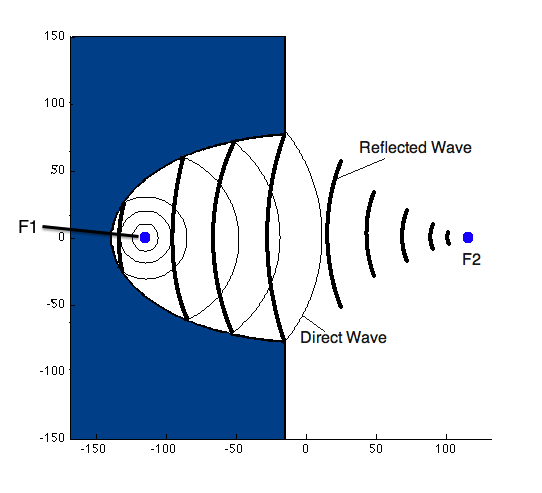
\includegraphics[scale=0.35]{lithotripter_schematic.png}\hspace{1mm}
b) 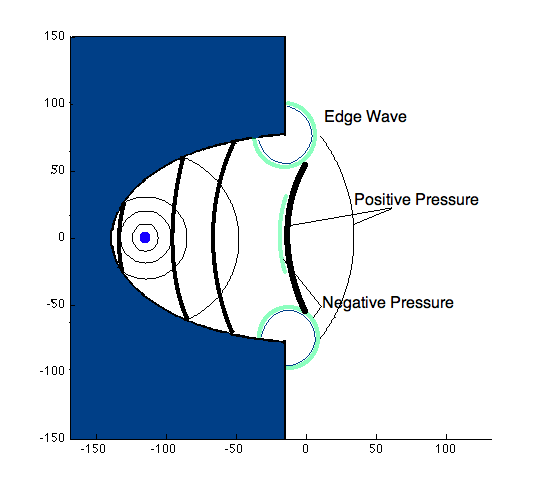
\includegraphics[scale=0.35]{lithotripter_edge_wave.png}
\end{center}
\caption{Cartoon of the Dornier HM3 Lithotripter.  In a) the spherical wave is generated at F1, reflects off the ellipsoid and the reflected wave focuses at F2.  In b) the diagram illustrates the creation of the edge waves at the corner of the ellipsoid and the contribution of negative pressure to the tail of the ESWT pressure wave.}
\label{fig:hm3_diagram}
\end{figure}

In addition to the HM3, we have also used the geometry of the
hand-held Sanywave device used by our collaborator Dr. Michael Chang.
Some sample calculations related to the study of HOs are presented in
\Sec{HO}.

In each case, the ESWT pressure wave form
that is generated has a similar shape. There is a sharp increase
in pressure from atmospheric pressure ($\sim0.1$MPa)
to a peak  pressure ranging from $35--100$
MPa over a very short rise time ($\sim10$ns), 
followed by a decrease in pressure to $\sim-10$
MPa over $\sim5 \mu$s. The negative fluid pressure in the tail can lead to
cavitation bubbles, as discussed below.

%Discuss shock wave profile?

Computational models for shock wave propagation and focusing can
aid in the study of ESWT.  In particular, there are many open
questions concerning the interaction of shock waves with complex
three-dimensional geometries such as bone embedded in tissue.
Because of the difference in material properties, a wave hitting
the tissue/bone interface will be partially reflected, and the
tranmitted wave will have a modified strength and direction of
propagation.  This can greatly affect the location and size of the
focal region as well as the peak pressure amplitude.  Moreover,
although the shock wave is primarily a pressure wave in soft tissue
(which has a very small shear modulus), at a bone interface 
mode conversion takes place and shear waves as well as compressional
waves are transmitted into the bone.  These shear waves may be
important in biological stimulation.  An additional effect is the
formation and collapse of cavitation bubbles that can cause tissue
damage.  While the shock wave is a compression wave, it is followed
by a rarefaction wave of expansion, and in the tail the fluid
pressure typically drops to negative values.  Reflection at interfaces
can lead to enhanced regions of expansion and to sufficiently
negative pressures that cavitation bubbles can form.

To better understand all of these effects, it is desirable to have a
three-dimensional computational model that can simulate the focusing of
nonlinear shock waves and their interaction with arbitrarily complex
interfaces between different materials.  

In this paper we present an approach to this problem that has allowed
the study of some of these issues in a simplified context.  In
particular, we consider an idealized situation in which soft tissue
is replaced by water, ignoring its viscoelastic properties, and
modeled by the nonlinear compressible Euler equations with the
Tamman or Tait equation of state.  Bone is modeled as an isotropic
and homogeneous linear elastic material.

In reality, soft tissue and bone are very complex multiscale materials
with microstructures, inhomogeneities, and anisotropic properties.
Any attempt to model the biological effect of shock wave propagation
through such materials may require a more sophisticated and detailed
model than used here.  However, we believe that many of the macro-scale
shock propagation issues discussed above can be adequately and most
efficiently studied with a simplified model of the form considered here,
since the dominant effect we hope to capture is the reflection and
transmission of waves at interfaces between materials.  

The compressible Euler equations with the Tamman equation of state (see
\Sec{eos_discussion}) in two-dimensional axisymmetric geometry is used to model the
intial formation of the focusing shock wave.  These initial conditions are
then fed into a code that uses a simpler nonlinear
model, the Tait equation of state,
in a three-dimensional simulation of the fluid.  The compressible fluid
equations are written using a Lagrangian formulation that easily couples to
the isotropic linear elasticity equations used in the bone-like material.
The resulting equations have the same form everywhere, with a different
stress-strain relationship in the different materials.

A high-resolution finite volume method is used to solve these equations.
We use the wave-propagation algorithms described in \cite{??}
and implemented in Clawpack \cite{claw.org.url}.  These are Godunov-type
methods for the hyperbolic system that use solutions to the Riemann problem
between adjacent grid cells to determine a set of waves used to update the
solution, and second-order correction terms with slope limiters are added to
resolve the nearly discontinuous shock waves with minimal smearing or
nonphysical oscillation.

These methods are used on a purely rectangular Cartesian grid.  Each
grid cell has associated with it a set of material parameters
determining the material in the cell, in a unified manner so that
both fluid and solid can be modeled.   Complex geometry is handled
by using appropriate averaged values of these parameters in cells
that are cut by the interface.  This is described further in \Sec{??}.
Averaging across the interface works quite well when the material properties
are sufficiently similar and in \Sec{??} we show that this is the case even
for fluid/solid boundaries of the type we consider.  

We also use patch-based adaptive mesh refinement (AMR) to concentrate
grid cells in regions where they are most needed to resolve features
of interest.  The Clawpack software contains AMR software in both
two and three space dimensions and this software has been used
directly for the two-dimensional axisymmetric computations of the
initial shock wave described in \Sec{??}.  For the three-dimensional
problem we have used ChomboClaw \cite{??}, an inteface between
Clawpack and the Chombo code developed at LBL \cite{chomboclaw}, which
provides an implementation of AMR on parallel machines using MPI.
Using ChomboClaw, the code originally developed using Clawpack was
easily converted into a code that was run on a TeraGrid machine at
Texas Advanced Computing Center (TACC) and tested using up to 128 processors.


Extensive laboratory experiments have been performed on
shock wave devices to measure the wave form of shock waves produced by
various devices, the shape of the focal region, the peak amplitudes of
pressure observed in these regions, and other related quantities.  Most of
these experiments have been done in a water tank where the shock wave
propagates and focuses in a homogeneous medium where measurements are easily
done, or with phantoms that are placed in the water as a proxy for bones or
kidney stones, with instrumentation such as pressure gauges or photographs
used to explore the interaction of the shock wave with the object.  In some
cases high-speed photographs of the shock wave have been obtained.
Creating phantoms from clear bi-refringent materials and using polarized
light it is even possible to photograph the shock wave propagating through
the object \cite{??}.  We have used some of these experiments to help
validate our numerical approach (see \Sec{??}).

Other researchers have also developed computational models for 
shock wave therapy and lithotripsy.
In prior work the pressure field has been modeled using linear and
nonlinear acoustics as well as the Euler equations with the Tait
equation of state.  Hamilton \cite{hamilton} used linear geometrical
acoustics, which holds under the assumption of weak shock strength,
to calculate the reflection of the spherical wave.  The diffraction
of the wave at the corner of the reflector was calculated using the
Kirchoff integral method.  Christopher's \cite{christopher_hm3}
model of the HM3 lithotripter used Hamilton's result as a starting
point and considered non planar sources.  Coleman et al \cite{coleman},
Averkiou and Cleveland \cite{cleveland_averkiou} used models based
on the KZK equation.  Tanguay \cite{tanguay} solved the full Euler
equations and incorporated cavitation effects as well as the edge
wave.

Our approach differs from these in that we consider the wave
propagation in both the fluid and solid by solving a single set of
equations that can model both materials.  This approach allows us
to investigate not only compression and tension effects of ESWT,
but also the propagation of shear waves in the solid.  Sapozhnikov
and Cleveland \cite{oleg_cleveland} have investigated the effect
of shear waves on spherical and cylindrical stones using linear
elasticity with a plane wave initial condition.  This initial
condition is an unfocused wave, which yields good results for small
objects, but would fail to capture the full ESWT pressure wave
interaction with three-dimensional bone geometries.

Summary of results in this paper....




\section{Model equations}
\label{sec:model_equations}
Much of the previous work on ESWT has been centered around the use of the Euler equations with the 
Tait or Tamman equations of state.  These equations of state are typically used for modeling underwater 
explosions like the spark plug source of the lithotripter device \cite{hamilton,toro_ivings}.  In this section 
we discuss the full Euler equations and proceed to show why the Tait equation of state is sufficient for 
modeling ESWT.  Since this equation of state is only a function of the density, $\rho$, we show how it 
can be modeled within the framework of linearized elasticity, which enables us to model both the fluid 
and solid with a single system of equations. 

In two space dimensions the Euler equations take the form
\begin{equation}
	\frac{\partial}{\partial t} q + \frac{\partial}{\partial x} f(q) + \frac{\partial}{\partial y} g(q) = 0,
	\label{eqn:euler2D}
\end{equation}
with 
\begin{equation}
	q = \left[ \begin{array}{c} \rho \\ \rho u \\ \rho v \\ E \end{array} \right  ], ~~~ 
	f(q) = \left[ \begin{array}{c} \rho u \\ \rho u^2 + p \\ \rho uv \\ u(E+p) \end{array} \right],~~~
	g(q) =  \left[ \begin{array}{c} \rho v \\ \rho uv \\ \rho u^2 + p \\ v(E+p) \end{array} \right].
\end{equation}
Here $u$ and $v$ denote the velocities in the $x$ and $y$ direction, respectively.  The total energy is $E 
= \rho e + \frac{1}{2}(u^2 + v^2)$, and the total enthalpy is $H = h + \frac{1}{2}(u^2 + v^2)$.

Several of the problems we investigated are axially symmetric and this enabled us to reduce the three-
dimensional equations to a two-dimensional form.  If we first rewrite the equations in cylindrical 
coordinates $(r,\theta,z)$ and then assume no variation and zero velocity in the $\theta$ direction, the 
system we obtain is reduced to two variables, $r$ and $z$.  
\begin{equation}
	\frac{\partial}{\partial t} \left[ \begin{array}{c} \rho \\ \rho u_r \\ \rho u_v \\ E \end{array} \right] +
	\frac{\partial}{\partial r} \left[ \begin{array}{c} \rho u_r \\ \rho u_r^2 + p \\ \rho u_r w_z \\ u_r(E+p) 
\end{array} \right] + 
	\frac{\partial}{\partial z} \left[ \begin{array}{c} \rho w_z \\ \rho u_r w_z\\ \rho w_z^2 + p \\ w_z(E+p) 
\end{array} \right ] = 
	\left[ \begin{array}{c} -(\rho u_r)/r \\ -(\rho u_r^2)/r \\ -(\rho u_r v_z) \\ u_r(E+p)/r \end{array} \right ],  
	\label{eqn:2daxisymeuler}
\end{equation}
where $u_r$ and $w_z$ denote the velocities in the $r$ and $z$ directions, respectively.  These 
equations are of the same form as (\ref{eqn:euler2D}), with the addition of geometric source terms that 
are a result of the variable transformation.

\subsection{Equation of State}
\label{sec:eos_discussion}
In order to solve the system (\ref{eqn:euler2D}) or (\ref{eqn:2daxisymeuler}), we need to close the 
system with a relation between the pressure and conserved variables.  We have used the Tait 
\cite{thompson} and Tammann \cite{ivings_toro} equations of state, which are applicable to a wide range 
of liquids.  It has been common practice to use the Tait EOS in shock wave therapy and lithotripsy 
models \cite{saito,nakahara_hugoniot}.  This may seem surprising considering the treatment relies upon 
shock waves to deliver energy and mechanical forces, which typically require a non-isentropic EOS.  
The Tammann equation of state is valid for non-isentropic flow and experiments have shown that two 
equations of state agree in the isentropic flow regime \cite{thompson}.  In the event that the shock is 
weak, or there is only a very small change in the entropy, an equation of state that only depends on the 
density, such as the Tait equation of state, can be used.  Several studies have indicated that in ESWT, 
there is no significant change in density or pressure as a result of the change of entropy across the 
shock \cite{nakahara} for pressures ranging from $1-200$ MPa.  This indicates that the use of the Tait 
equation of state should be sufficient for the study of ESWT.

The Tait equation of state is
\begin{equation}
	p = p(\rho) = B\left[ \left(\frac{\rho}{\rho_0}\right)^n - 1\right], 
	\label{eqn:taiteos}
\end{equation}
where B is a pressure constant that is a weak function of entropy, but is typically treated as a constant, 
$n$ is a constant playing a similar role to that of $\gamma$ in the ideal gas law, $\rho$ is the density, 
and $p$ the pressure.

The Tammann equation of state can be written as
\begin{equation}
	p = p(\rho, e) = (\gamma - 1)\rho e - \gamma p_{\infty},
	\label{eqn:tammaneos}
\end{equation}
where $p$,$\rho$ and $e$ are the pressure, density and specific internal energy, respectively.  The 
values in water for the pressure constant, $p_c$, and polytropic constant, $\gamma$, are the same as 
$B$ and $n$ in the Tait equation of state.  This equation is similar to the ideal gas law, and reduces to 
the ideal gas law in the case where $p_{\infty} = 0$ and $ 1 < \gamma < 2$.

If it is possible to use the Tait EOS in our model, the equations (\ref{eqn:1dlageulfixgrid}) can be further 
simplified, reducing the computational complexity of our simulations.  Therefore, we performed a 
numerical investigation of the propagation of a shock wave when modeled by both the Tammann and 
Tait equation of state.  Figure \ref{fig:tait_tamman} a) shows the result from one experiment where a 
shock wave with peak over pressure of $\approx 180$ MPa has propagated through water.  The blue 
wave represents the result from solving with the Tammann equation of state and the red represents the 
solution with the Tait equation of state, the pressure profiles are nearly identical.  This gives us 
confidence that the calculations we are interested in can be done by solving the Euler equations with the 
Tait equation of state, and we can therefore neglect the equation for energy
\begin{equation}
	\frac{\partial}{\partial t} \left[ \begin{array}{c} \rho \\ \rho u \\ \rho v \end{array} \right] +
	\frac{\partial}{\partial x} \left[ \begin{array}{c} \rho u_r \\ \rho u^2 + p \\ \rho u v \end{array} \right] + 
	\frac{\partial}{\partial y} \left[ \begin{array}{c} \rho w_z \\ \rho u v\\ \rho v^2 + p \end{array} \right ] = 
	\left[ \begin{array}{c} 0 \\ 0 \\0  \end{array}\right ]. 
	\label{eqn:isentropic}
\end{equation}

\begin{figure}
%\begin{center}
a)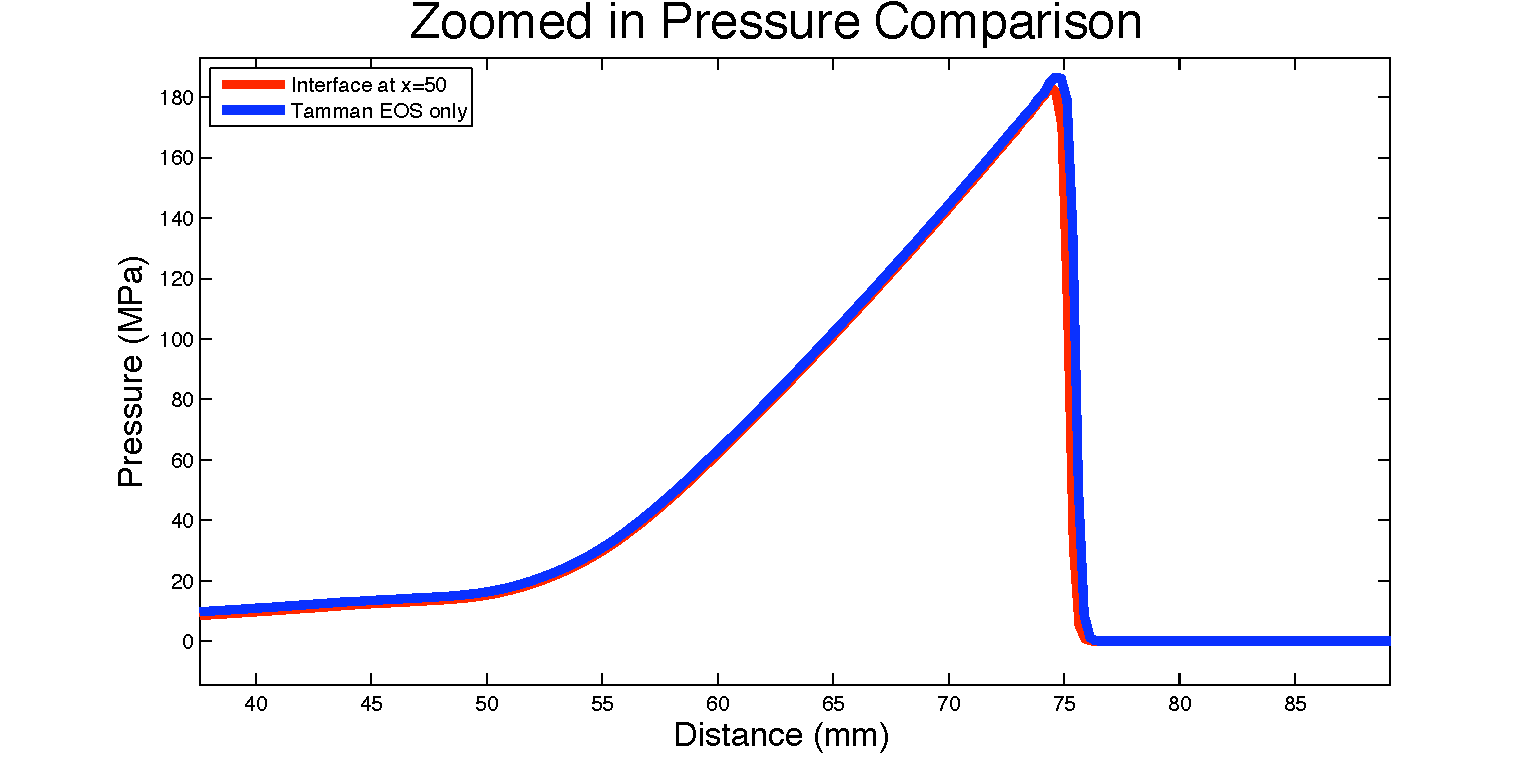
\includegraphics[height=1.5in, width=2in]{tamman_tait_pressure_zoom.pdf}
b)\includegraphics[height=1.5in, width=2in]{lagrangian_eulerian.pdf}
\caption{a) Comparison of a pressure wave calculation performed using both the Tait and Tammann 
equations of state.  The results are nearly identical. b) Comparison of the pressure pulse at F2 obtained 
in the Euler calculation (red dashed curve) and the Lagrangian calculation (blue curve).  It is clear that 
the two sets of equations give good agreement.  The wave in the Lagrangian case is slightly attenuated, 
but this may be due to error in initializing the calculation. In these calculations $\Delta x = 0.5 mm$.}
\label{fig:tait_tammann}
%\end{center}
\end{figure}



%\begin{figure}[ht]
%\begin{center}
%\includegraphics[scale=0.25]{euler_init/crop/lagrangian_eulerian.pdf}
%\caption{Comparison of the pressure pulse at F2 obtained in the Euler calculation (red dashed curve) 
and the Lagrangian calculation (blue curve).  It is clear that the two sets of equations give good 
agreement.  The wave in the Lagrangian case is slightly attenuated, but this may be due to error in 
initializing the calculation. In these calculations $\Delta x = 0.5 mm$.}
%\label{fig:eul_lag_comp}
%\end{center}
%\end{figure}

\subsection{Elasticity equations}
\label{sec:elasticity}
In the case of infinitesimal or small displacements, it is possible to write the elasticity equations as 
\begin{align}
 \epsilon_t - u_x &= 0 \label{eqn:nlelast}\\
 \rho_0 u_t - \sigma(\epsilon)_x &= 0  \notag\\
\end{align}
where the higher order terms in the deformation tensor have been neglected.  This form of the equations 
still allows for nonlinear behavior to be incorporated through the stress-strain relationship, $
\sigma(\epsilon)$.  We take advantage of this formulation in order to incorporate the nonlinear Tait 
equation of state in the fluid. 

In the case of a fluid where the shear modulus is zero, the stress tensor can be written as $
\sigma(\epsilon) = -pI$, where $p$ is the pressure in the fluid and $I$ is the identity matrix.  In the case of 
ESWT, the pressure only depends on changes in the density, and we can rewrite $p(\rho)$ as a function 
of the strain tensor $\epsilon$.  In the case of small deformations, we have that 
\begin{equation}
\rho = \frac{\rho_0}{\det(F)} = \frac{\rho_0}{1+tr(\epsilon)},
\end{equation}
where $F$ is the deformation gradient tensor.

If we plug this into the Tait equation of state (\ref{eqn:taiteos}) we get
\begin{equation}
p(\rho) = p(\epsilon) = B\left[ \left(\frac{1}{1 + tr(\epsilon)}\right)^n - 1\right].  
\end{equation} 
Therefore, in the fluid, we get the following for our stress-strain relationship 
\begin{equation}
\sigma(\epsilon) = -(B\left[ \left(\frac{1}{1 + tr(\epsilon)}\right)^n - 1\right]) I
\end{equation} 

This is only valid in the case where the displacements are small, so we calculated the maximum value of 
the displacements in a two-dimensional axisymmetric calculation with the Euler equations.  We found 
that for the maximum peak pressure of 50MPa, the corresponding maximum velocity was (look up 
numerical values from the calculation) $10^{-3}$m/s.  We then calculated the maximum displacement by 
integrating the velocity over the time step of the calculation and found this to be on the order of 
$10^{-5}$mm.  It is therefore reasonable to assume that the density in each grid cell is essentially 
constant, $\rho = \rho_0$ and that the Lagrangian framework of the elasticity equations will be valid for 
the fluid.  To test this, we took the same initial condition for the 2D axisymmetric Euler equations with the 
Tamman equation of state and the corresponding 2D axisymmetric Lagrangian form of the equations 
with the Tait equation of state and measured the pressure at the focus, F2.  The results in Figure 
\ref{fig:tait_tamman} b) demonstrate reasonably good agreement between the two cases, but the 
Lagrangian form is slightly attenuated.  This may be due to conversion of the initial condition from the 
conserved variables in the Euler equations (\ref{eqn:2daxisymeuler}) to those in the elasticity equations 
(\ref{eqn:elastiic}).

Since the displacements are so small, it may be reasonable to use a linearized version of the Tait 
equation of state in our calculations, so then we would be able to simply use the linear elasticity 
equations.  If we assume a small perturbation to the strain, $\epsilon + \delta \epsilon$, we can write the 
(\ref{eqn:taiteos}) as
\begin{equation}
	p(\epsilon) = p_0 + p'(\delta \epsilon) \epsilon + \frac{p''(\delta \epsilon)}{2} \epsilon^2 + 
\text{ H.O.T. }
	\label{eqn:tait_taylor}
\end{equation}
What we call the linear Tait EOS is just the first two terms of (\ref{eqn:tait_taylor}) and the quadratic Tait 
EOS is the first three terms.  We found that for smaller amplitude waves, the linear Tait EOS is insufficient 
for predicting the correct arrival time or amplitude.  If we include the quadratic term, then we can 
accurately determine the arrival time, but the amplitude is still incorrect.  As we increase the amplitude of 
the pressure wave, i.e. there is a larger jump in pressure across the shock, neither the linear nor 
quadratic EOS can capture the correct arrival time or amplitude.  This is demonstrated in Figure
\ref{fig:tait_linearization}.

\begin{figure}
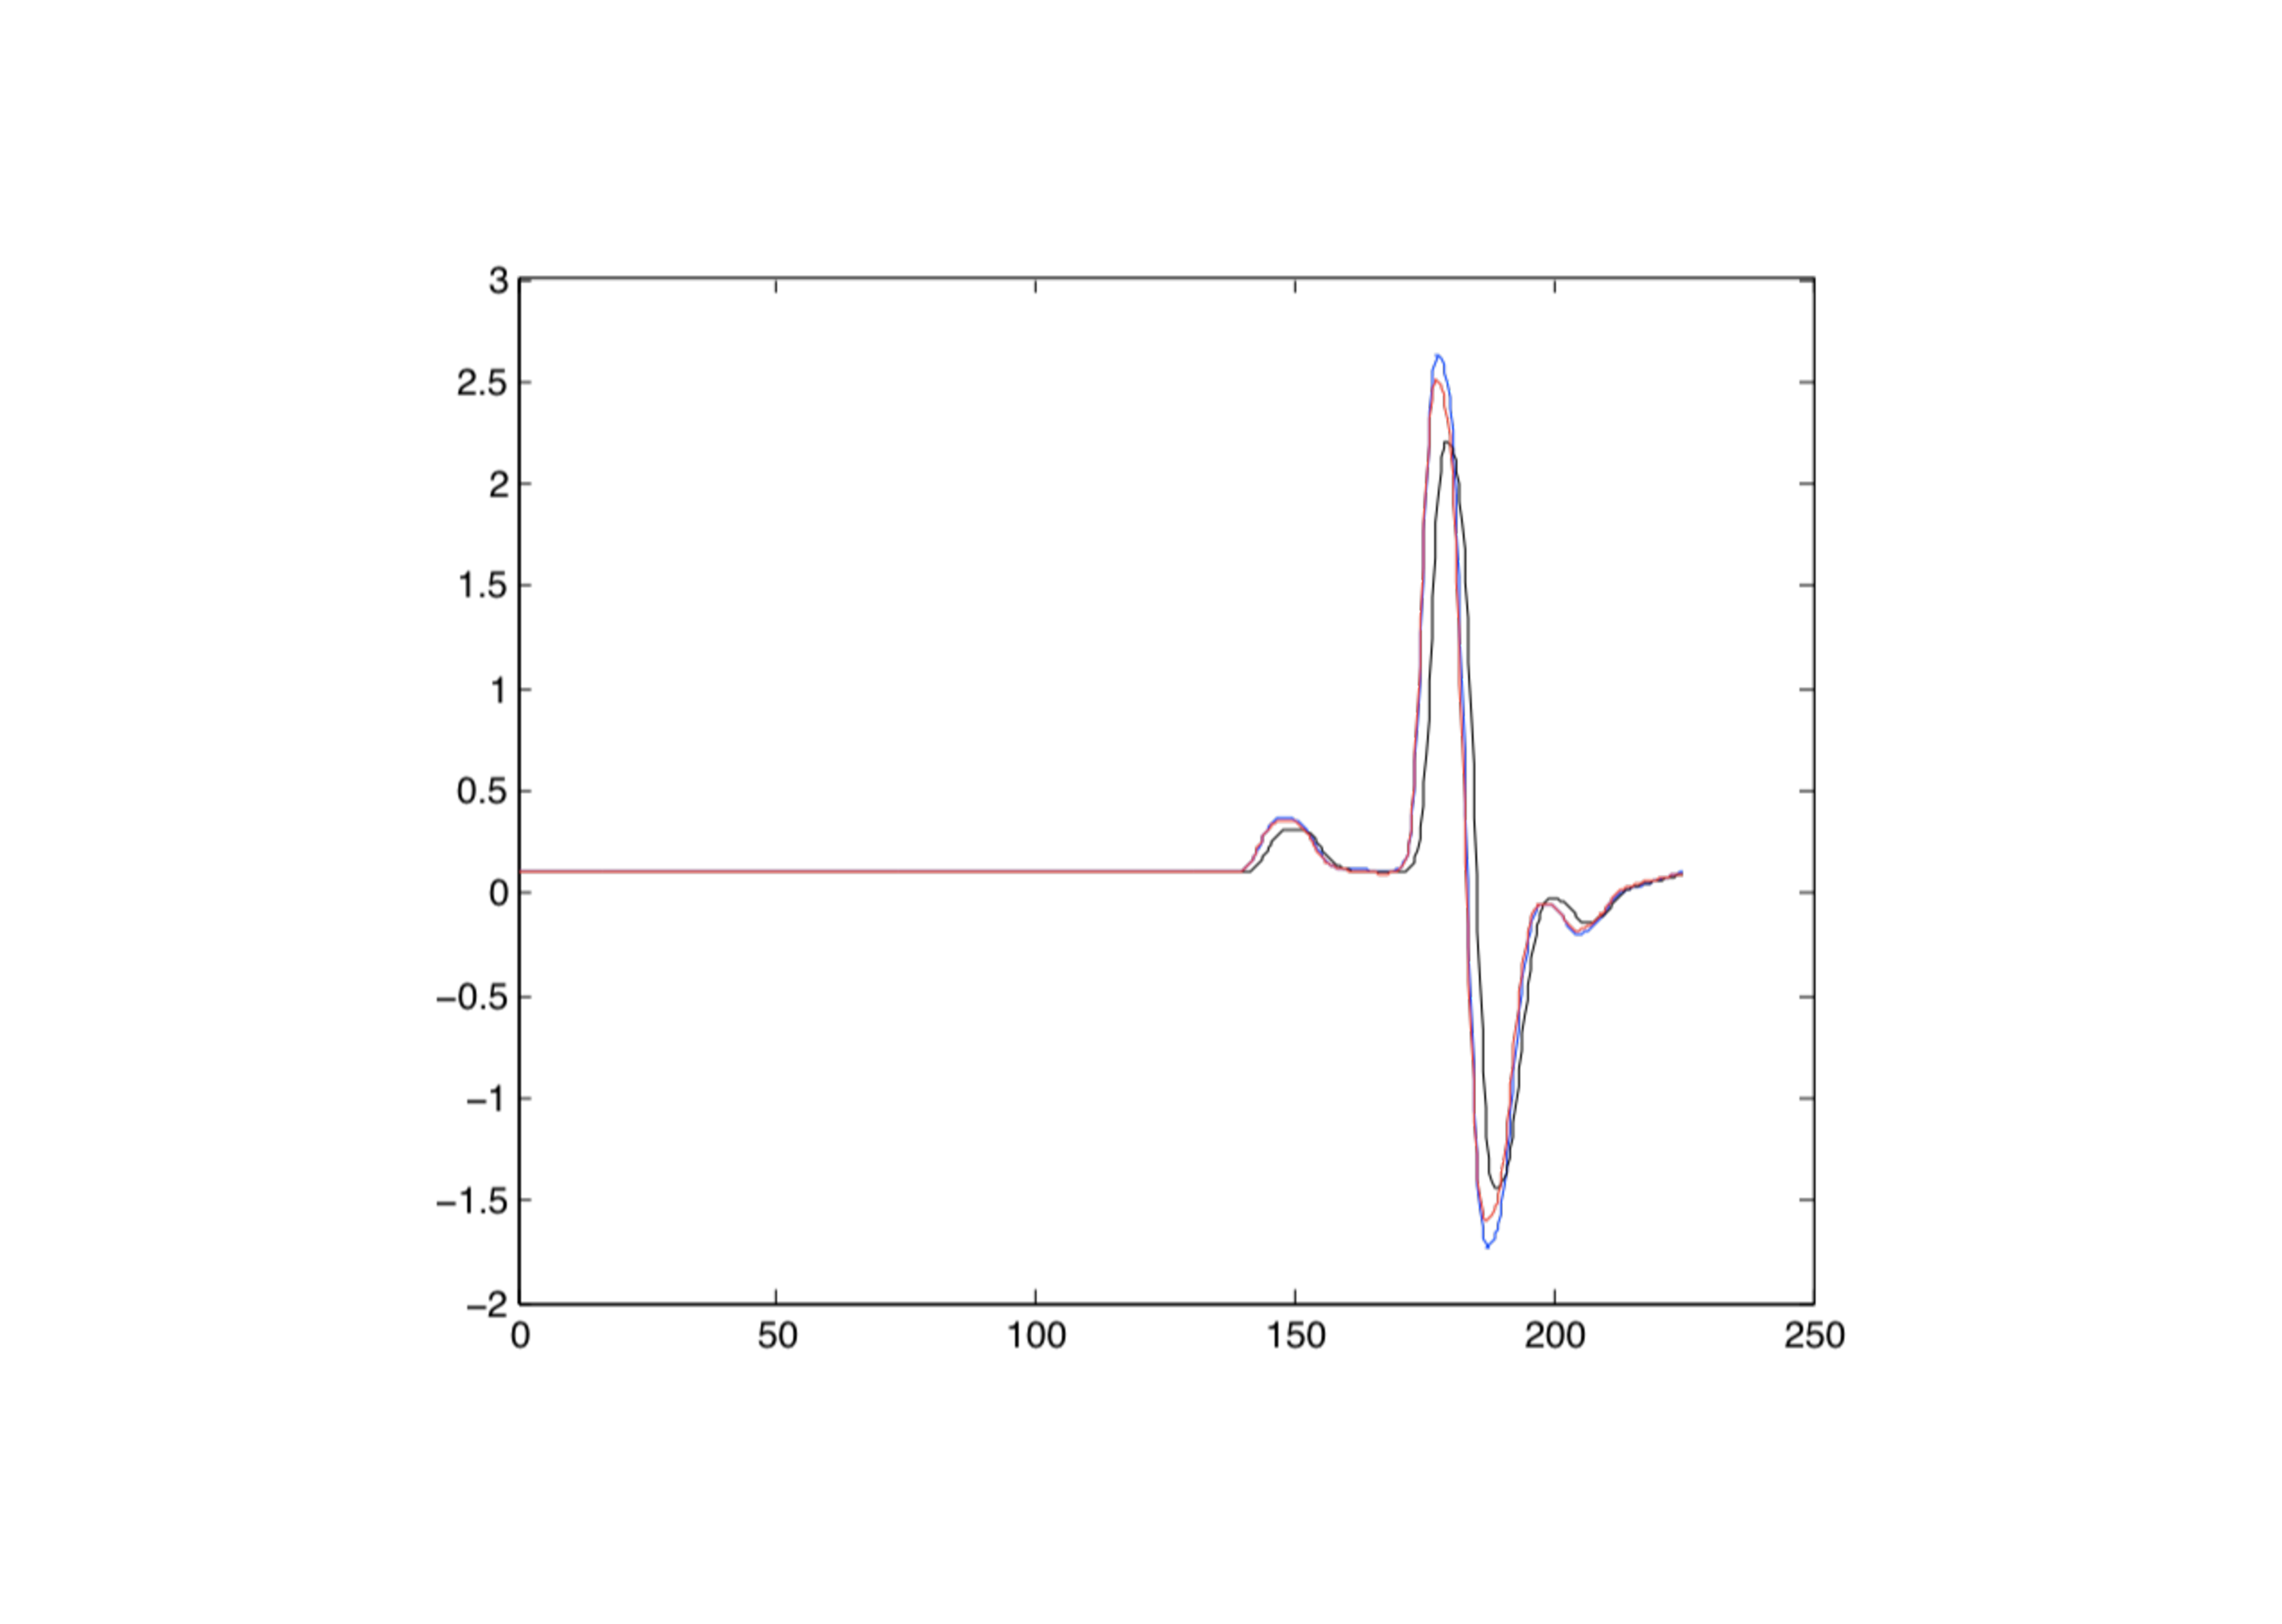
\includegraphics[width=2in]{linearization_small_amp.pdf}
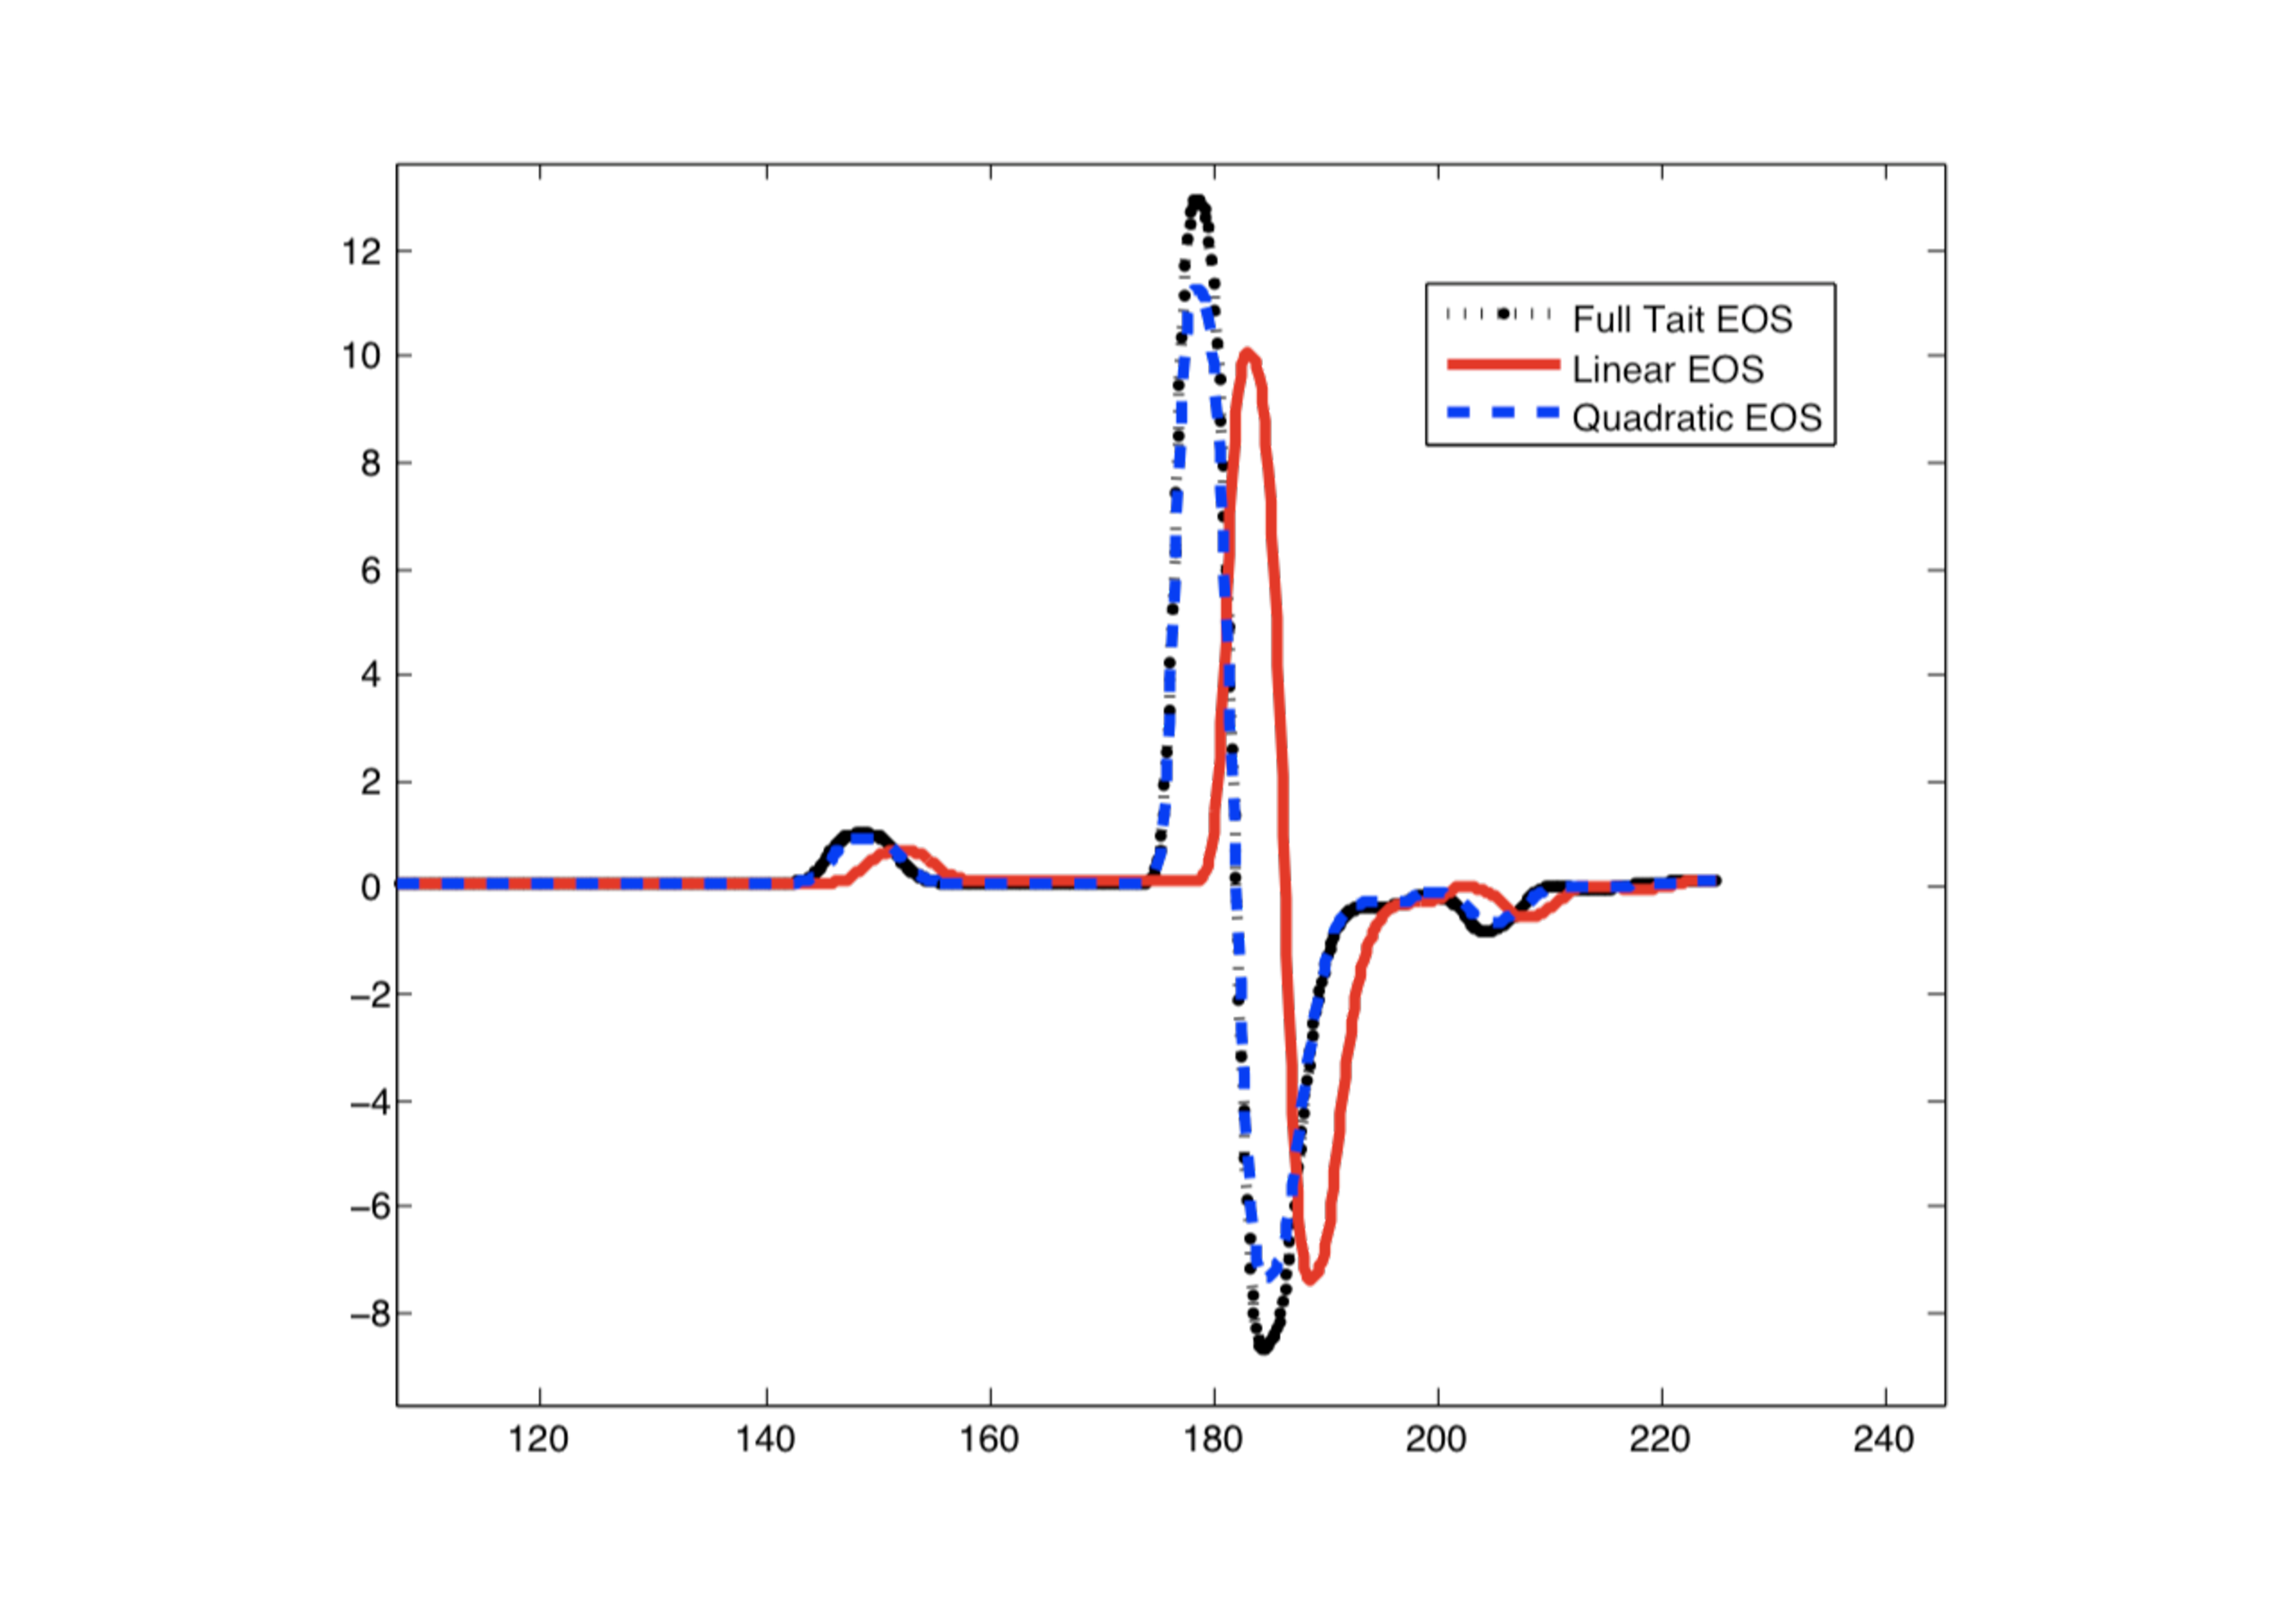
\includegraphics[width=2in]{med_amplitude_comp.pdf}
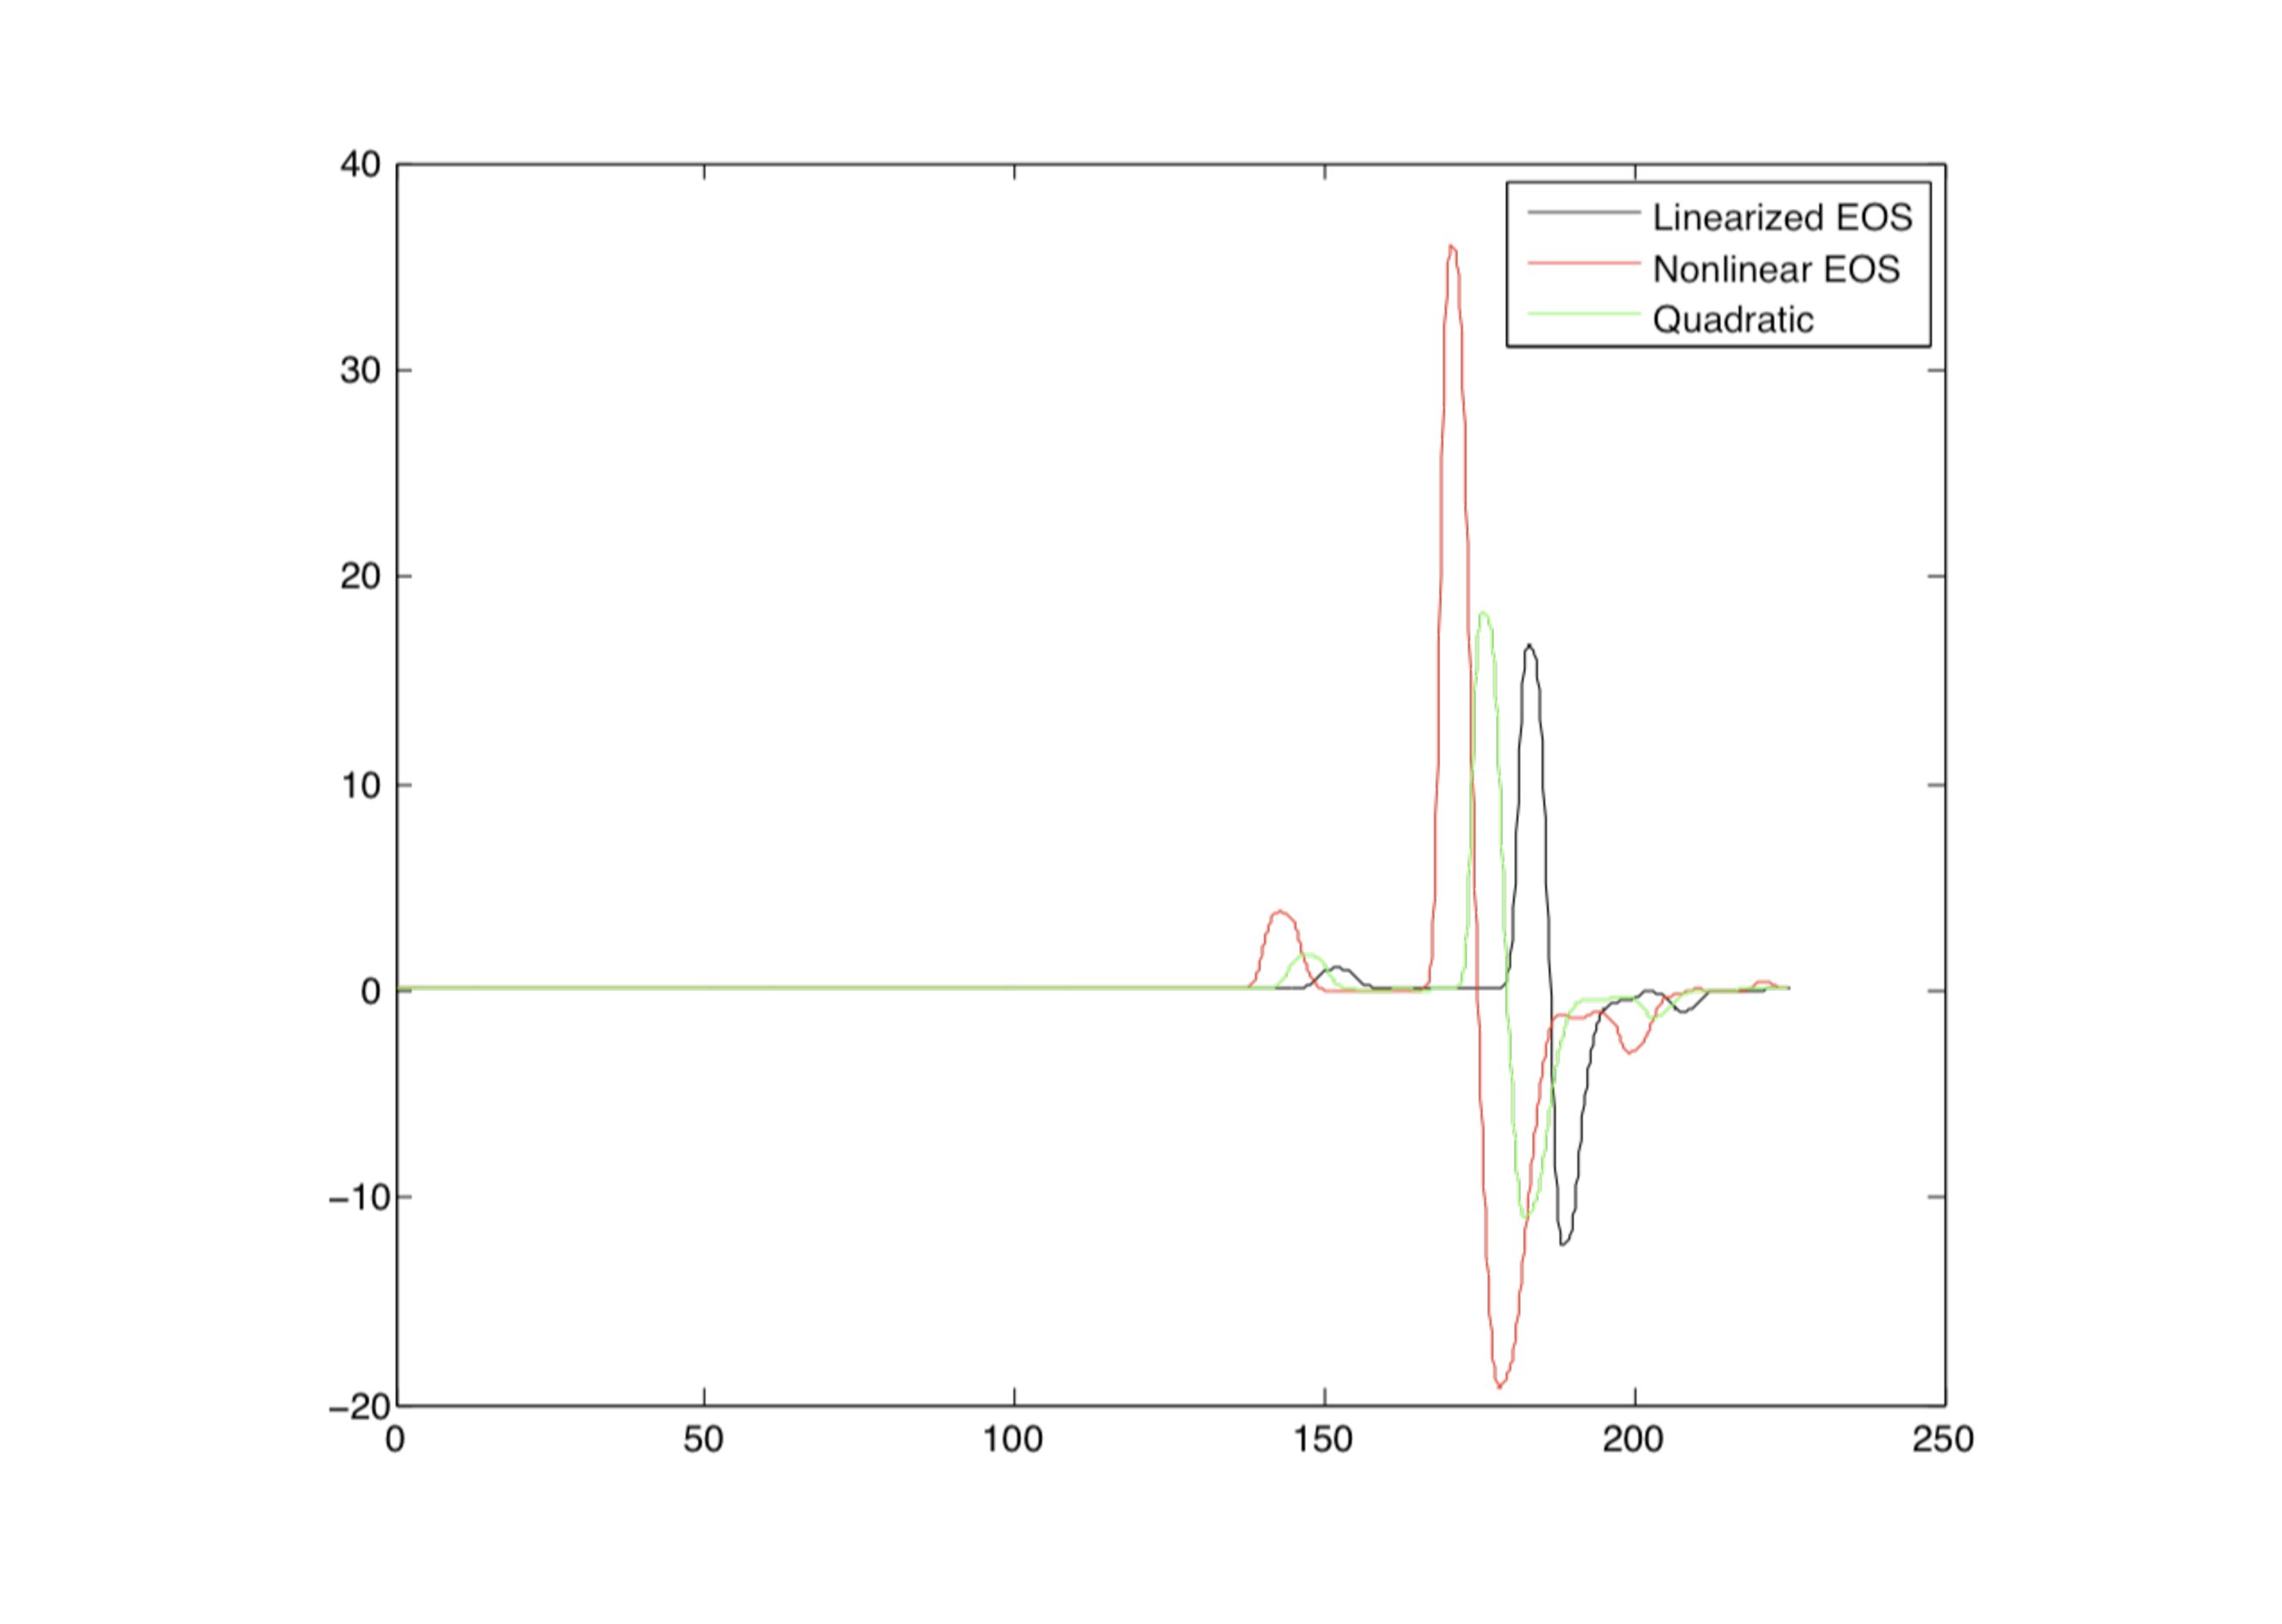
\includegraphics[width=2in]{higher_amplitude.pdf}
\label{fig:tait_linearization}
\caption{I will make these look better later if we decide to include them.  I'm trying to think of a better 
plot... maybe error vs. amplitude or something like that to just summarize the results}
\end{figure}

For the linear isotropic solid, we use Hooke's law
\begin{align*}
\sigma^{11} &= C_{11} \epsilon^{11} + C_{12} \epsilon^{22} + C_{13} \epsilon_{33} \\
\sigma^{22} &= C_{21} \epsilon^{11} + C_{22} \epsilon^{22} + C_{23} \epsilon^{33}  \\
\sigma^{33} &=C_{31} \epsilon^{11} + C_{32} \epsilon^{22} + C_{33} \epsilon^{33}  \\
\sigma^{12} &= C_{44} \epsilon^{12} \\
\sigma^{13} &= C_{55} \epsilon^{13}\\
\sigma^{23} &=  C_{66} \epsilon^{23}. \\
\end{align*}
where the scalar coefficients $C_{ij}$ are determined by the properties of the material being modeled.  
The parameters used for the bone model were found in \cite{burr}.

With these two stress-strain relations and the methodology discussed in \Sec{numerics}, we are able to 
model ESWT with one system of equations.

%\subsection{Comparison of Lagrangian and Eulerian Solution}
%\label{sec:lag_eul_comp}
%Given the result in Figure \ref{fig:tait_tammann} a), combined with the small displacements in our 
model, we are confident that the two systems of equations should agree for the weak shocks present in 
ESWT.  We performed an axisymmetric calculation with the Euler equations using the Tammann 
equation of state to generate an initial condition for the experiment.  We then measured the focused 
wave form at $x=115.0$ for both the Eulerian and Lagrangian form of the equations.  In Figure 
\ref{fig:tait_tammann} b) we see that the two models give nearly the same solution, however, the wave 
from the Lagrangian calculation has been slightly attenuated.


\section{Numerical Methodology}
\label{sec:numerics}
We used the wave-propagation algorithms described in \cite{rjl_book} and implemented in CLAWPACK 
\cite{clawpack} to solve the system \ref{sys:nlelast}.  In this section we provide the basic details of the 
numerical methodology and approximate solution to the Riemann problem with a spatially-varying flux 
function, similar to what was done in \cite{rjl_nonlinear}  We also discuss computational issues that 
necessitate the use of Adaptive Mesh Refinement. 

\subsection{Approximate Riemann Solver}
\label{sec:riemann_solver}
In order to apply the high-resolution wave propagation algorithms described in 
\cite{rjl_book,rjl_nolnlinear} to equations (\ref{sys:nlelast}), we must first determine the solution to the 
Riemann problem.  Recall that the Riemann problem is the initial value problem for a hyperbolic system 
of conservation laws, 
$$
	q_t + f(q)_x = 0, 
$$
with special initial data consisting of two constant states separated by a discontinuity
$$
	    q_{0}(x) = \begin{choice} q_l &\text{if}~x<0 \\
                    q_r &\text{if}~x>0 \end{choice}.
$$
For nonlinear systems of equations, such as (\ref{eqn:nlelast}) this is often most efficiently done through 
the use of an approximate Riemann solver \cite{rjl_book}.  

The approximate Riemann solver is developed using an approach that has been successfully applied to 
conservation laws of the form
\begin{equation}
q_t + f(q,x)_x =0,
\end{equation}
where $f(q,x)$ is a spatially-varying flux function.  The flux function is how we incorporate different 
equations of state, or stress-strain relations, to model the different materials.  The Riemann problem 
between computational grid cells $i-1$ and $i$ is based on two flux functions $f_{i-1}(q)$ and $f_i(q)$, 
as well as the data $Q_{i-1}$ and $Q_i$.  In the case considered below, there are always at least two so-
called P-waves in the Riemann solution.  One wave $\mathcal{W}^1$ propagating to the left with speed 
$s^1=-c_p < 0$ and $\mathcal{W}^2$ propagating to the right with speed $s^2 = c_p > 0$.  In the solid 
there may be four additional shear or S-waves propagating at speeds $\pm c_s$.  If the shear modulus 
is zero, there will be 7 zero-speed stationary waves, otherwise there will only be 3.  These waves are 
taken to be of the form $\mathcal{W}^j = \alpha^j r^j$ for $j=1\dots9$.  In our case, the vectors $r^j$ are 
taken to be the eigenvectors of a linearized problem $f^{\prime}(q,x)$ and $\alpha^j$ are scalar 
coefficients.  The $\alpha^j$ are typically determined by solving $Q_i - Q_{i-1} = R {\bf \alpha}$, where R 
is the matrix of eigenvectors $r^j$. However, since we have a spatially-varying flux function, we 
determine these scalars by solving $f_i(Q_i) - f_{i-1}(Q_{i-1}) = R {\bf \beta}$.  Then, using $\beta^j$ we 
get $\alpha^j = \beta^j/s^j$.  The full details of the so-called {\it f-wave decomposition} can be found in 
\cite{rjl_bale_rossmanith}.

In general, the solution to the Riemann problem will have the structure detailed in Figure 
\ref{fig:riemann_tait_elas}.  This particular case shows the solution where two neighboring grid cells 
have different stress-strain relationships. 
(explain in greater detail and include diagram)

\subsection{Solution of the Riemann Problem for 3D Nonlinear Elasticity}
\label{sec:3Delasticity}
The full three-dimensional system of equations for the Isentropic Euler equations in Lagrangian 
coordinates is 
\begin{align}
(\epsilon_{11})_t &= \frac{\partial u}{\partial x}\notag\\
(\epsilon_{22})_t &= \frac{\partial v}{\partial y}\notag\\
(\epsilon_{33})_t &= \frac{\partial w}{\partial z}\notag\\
(\epsilon_{12})_t &= \frac{1}{2}\left(\frac{\partial u}{\partial y} + \frac{\partial v}{\partial x}\right)\notag\\
(\epsilon_{23})_t &= \frac{1}{2}\left( \frac{\partial v}{\partial z} + \frac{\partial w}{\partial y}\right)\label{eqn:
3dlgeulsys}\\
(\epsilon_{13})_t &= \frac{1}{2}\left( \frac{\partial u}{\partial z} + \frac{\partial w}{\partial x}\right)\notag\\
\rho u_t &= \frac{\partial \sigma_{11}}{\partial x} +\frac{\partial \sigma_{12}}{\partial y} +  \frac{\partial 
\sigma_{13}}{\partial z}\notag\\
\rho v_t &=   \frac{\partial \sigma_{12}}{\partial x} +\frac{\partial \sigma_{22}}{\partial y} + \frac{\partial 
\sigma_{23}}{\partial z}\notag \\
\rho w_t &=  \frac{\partial \sigma_{13}}{\partial x} + \frac{\partial \sigma_{23}}{\partial y} + \frac{\partial 
\sigma_{33}}{\partial z}.\notag
\end{align}
We can write this system in the form 
\begin{equation}
	q_t - A(x,y,z) q_x + B(x,y,z) q_y + C(x,y,z) q_z = 0, 
\end{equation}
where $A$,$B$ and $C$ are the Jacobians of the flux functions in the $x$, $y$ and $z$ directions 
respectively.  For the multi-dimensional methods implemented in CLAWPACK, we need the solution to 
the Riemann problem along slices in each coordinate direction.  Here we provide the details for the 
solution in the $x$-direction, but the solution in the $y$ and $z$ directions are similar with appropriate 
perturbations to the $B$ and $C$ matrices. 

The corresponding Jacobian for this system in the $x$-direction is
\begin{equation}
A(q) = f^{\prime}(q) = -\left(\begin{array}{ccccccccc}0&0&0&0&0&0&\frac{1}{\rho}&0&0\\ 
0&0&0&0&0&0&0&0&0\\0&0&0&0&0&0&0&0&0\\0&0&0&0&0&0&0&\frac{1}{2\rho}&0\
\0&0&0&0&0&0&0&0&0\\0&0&0&0&0&0&0&0&\frac{1}{2\rho}\\ \sigma^{11}_{\epsilon^{11}} & 
\sigma^{11}_{\epsilon^{22}} &\sigma^{11}_{\epsilon^{33}} & 0 &0 &0 &0&0&0\\0&0&0&
\sigma^{12}_{\epsilon^{12}}&0&0&0&0&0\\0&0&0&0&0&\sigma^{13}_{\epsilon^{13}}&0&0&0 \end{array} 
\right)
\label{eqn:jac3dlgeul}
\end{equation}
The Jacobians in the $y$- and $z$- directions are similar with the entries perturbed appropriately. 

We have made use of the fact that the derivative of $\sigma^{11}$ with respect to the shear strain will be 
zero in either the Euler or elastic equations.  Similarly, the derivative of $\sigma^{12}$ or $\sigma^{13}$ 
will be non-zero only when taken with respect to the shear strains $\epsilon_{12}$ and $\epsilon^{13}$, 
respectively.

The eigenvalues for system (\ref{eqn:jac3dlgeul}) are
\begin{equation}
\lambda^{1,2} = \left (\pm \sqrt{\frac{\sigma^{11}_{\epsilon^{11}}}{\rho_0}}\right); ~~\lambda^{3,4} = \pm 
\sqrt{\frac{\sigma^{12}_{\epsilon^{12}}}{2\rho_0}}; ~~\lambda^{5,6} = \pm 
\sqrt{\frac{\sigma^{13}_{\epsilon^{13}}}{2\rho_0}}; ~~\lambda^{7,8,9}=0.
\label{eqn:3dlgeuleval}
\end{equation}

The corresponding eigenvectors for system (\ref{eqn:jac3dlgeul}) are
\begin{equation}
\left ( \begin{array}{c} 1\\0\\0\\0\\0\\0\\ \pm\sqrt{\rho_0 \sigma^{11}_{\epsilon_{11}}}\\ 0\\0
\end{array}
\right ),
\left ( \begin{array}{c} 0\\0\\0\\1\\0\\0\\0\\\pm \sqrt{2 \rho_0 \sigma^{12}_{\epsilon^{12}}}\\0
\end{array}
\right),
\left ( \begin{array}{c} 0\\0\\0\\0\\0\\1\\0\\0\\ \pm\sqrt{2 \rho_0 \sigma^{13}_{\epsilon_{13}}}
\end{array}
\right ),
\left ( \begin{array}{c}-\frac{\sigma^{11}_{\epsilon^{22}}}{\sigma^{11}_{\epsilon^{11}}}\\1\\0\\0\\0\\0\\0\\0\\0
\end{array}
\right ),
\left ( \begin{array}{c}-\frac{\sigma^{11}_{\epsilon^{33}}}{\sigma^{11}_{\epsilon^{11}}}\\0\\1\\0\\0\\0\\0\\0\\0
\end{array}
\right ),
\left ( \begin{array}{c}0\\0\\0\\0\\1\\0\\0\\0\\0
\end{array}
\right ).
\label{eqn:3dlgeulevec}
\end{equation}


The weights that we need to determine the wave strengths in the wave propagation algorithm found by 
solving $R \beta = f(Q_r) - f(Q_l)$ are found by solving
\begin{equation}
 \left ( \begin{array}{ccccccccc} 
 1& 0&0&1& 1&0&0&0& 1\\ 
 0&0 &0& -\frac{\sigma^{11}_{\epsilon^{11}}}{\sigma^{11}_{\epsilon^{22}}}& 0& 0&0&0&0 \\ 
 0&0 &0&0& -\frac{\sigma^{11}_{\epsilon^{11}}}{\sigma^{11}_{\epsilon^{33}}}&0&0&0&0 \\ 
0&1&0&0&0&0&0&1&0\\ 
 0&0&0&0&1 &0&0&0&0\\ 
 0&0&1&0&0&0&1&0&0\\
-\sqrt{\sigma^{11}_{\epsilon^{11}}\rho_0}& 0& 0& 0& 0& 0& 0&0&\sqrt{\sigma^{11}_{\epsilon^{11}}
\rho_0}\\ 
 0& -\sqrt{2\rho_0 \sigma^{12}_{\epsilon^{12}}} &0&0& 0& 0& 0 & \sqrt{2 \rho_0 
\sigma^{12}_{\epsilon^{12}}} &0 \\ 
 0& 0&-\sqrt{2\rho_0 \sigma^{13}_{\epsilon^{13}}} &0& 0& 0& \sqrt{2 \rho_0\sigma^{13}_{\epsilon^{13}}} 
&0 &0 \end{array}
\right )  \left ( \begin{array}{c} \beta^1\\ \beta^2 \\ \beta^3 \\ \beta^4\\ \beta^5\\ \beta^6 \\ \beta^7 \\ \beta^8 \\ 
\beta^9
\end{array}
\right ) = \left ( \begin{array}{c} f^1\\ f^2 \\ f^3 \\ f^4\\ f^5 \\f^6 \\f^7\\f^8\\f^9
\end{array}
\right ). 
\label{eqn:2dlgeulfwave}
\end{equation}

The solution of the Riemann problem shows that we should expect 9 waves.  We will get two P-waves 
that travel at the speed $\pm c_p$, four S-waves with speeds $\pm c_s$ and 3 stationary waves.  In the 
case of a fluid, there are no S-waves, so we get seven stationary waves.  For the wave-propagation 
algorithms implemented in CLAWPACK, we only use the waves with non-zero speeds for the updates.

\subsection{Transverse solvers}
The method described here is based on propagating waves normal to each interface.  In reality, the 
waves will propagate in a multidimensional manner and affect cell averages in cells above and below 
those that are directly adjacent to the interface.  In order to include these transverse effects, each 
fluctuation is split into two transverse fluctuations.  This transverse decomposition of the fluctuations can 
be viewed as solving a second Riemann problem in the transverse direction, even though it is not based 
on left and right states as we normally think of for a Riemann solver.  Once we have determined the 
transverse fluctuations, they can be used to update the fluxes obtained by solving the original Riemann 
problem.  The transverse correction terms also have the effect of improving the stability limit, allowing for 
a Courant number of 1, relative to the maximum wave speed in any direction. 

(Could you suggest the level of detail that should be provided here?)

\subsection{Wave speeds}
\label{sec:wavespeeds}
Since we have rewritten the equations in a Lagrangian frame, we checked to be sure that the new sound 
speeds, or eigenvalues for our Jacobian, are correct.  In the case of the Euler equations with the Tait 
equation of state, $p(\rho) = p(\epsilon) = B[(\frac{1}{(1+\epsilon^{11} + \epsilon^{22} + 
\epsilon^{33})}^{n} - 1]$, we get the following
\begin{align}
     \sigma_{\epsilon^{11}} &= B n \left( \frac{1}{(1+\epsilon^{11} + \epsilon^{22} + \epsilon^{33})} 
\right )^{n +1} \notag\\
     			&= B n \frac{1}{(1+\epsilon^{11} + \epsilon^{22} + \epsilon^{33})} \left( \frac{1}{(1+
\epsilon^{11} + \epsilon^{22} + \epsilon^{33})} \right )^{n} \label{eqn:sigepstait}\\
			&=  \frac{1}{(1+\epsilon^{11} + \epsilon^{22} + \epsilon^{33})} n (p + B).\notag
\end{align}
If we then substitute $\rho(t) \approx \rho_0$ into our formula for the eigenvalues (\ref{eqn:sigepstait}), 
we get the following for our wave speeds 
\begin{equation}
	\pm \sqrt{\frac{n (p+B)}{\rho_0}}.
\label{eqn:lagisenspeed}
\end{equation}
In the standard form of the isentropic Euler equations, we would expect eigenvalues of the form 
\begin{equation}
	\lambda^{1,2} = u \pm c_p,
\end{equation}
for the acoustic wave speeds, where $u$ is the velocity of the fluid particles and $c_p$ is the speed of 
sound in the fluid.  As demonstrated in Section \Sec{??}, the velocities of the fluid particles are small, 
with a maximum value on the order of $10^{-3}$m/s directly behind the shock.  As a result, we can 
neglect the particle velocity in our computation without much of an error and then the wave speeds 
above agree with those from the isentropic Euler equations. Since fluids do not support shear stress the 
s-wave speed is zero.


For elasticity if we assume that the density $\rho$ is constant throughout a specific material, but can still 
vary spatially, and denote it $\rho_0$, then the eigenvalues are\\
\begin{equation}
\lambda^{1,2} = \left[\pm \sqrt{-\frac{\sigma_{\epsilon^{11}}}{\rho_0}}\right],
\end{equation}
where $\sigma_{\epsilon^{11}} = (\lambda+2\mu)$.  This means that we have
\begin{equation}
\lambda^{1,2} = \pm \sqrt{\frac{\lambda+2 \mu}{\rho_0}},
\end{equation}
which are the correct sound speed for the p-waves in a linearly elastic medium.  For the s-waves we get
\begin{equation}
\lambda^{3,4} = \pm \sqrt{\frac{\sigma^{12}_{\epsilon^{12}}}{2\rho_0}} = \sqrt{\frac{\mu}{\rho_0}},
\end{equation}
which is the correct speed for the s-waves in the $x-y$ direction.  The case works out similarly for the $x-
z$ direction. 
%This section may not be necessary if it is more fully described above
%\subsection{Spatially-varying $\sigma(\epsilon)$}
%\label{sec:spatially_varying}
\subsection{Axisymmetric form of the equations}
\label{sec:axisym}
We used the two-dimensional axisymmetric form of the equations to generate and initial condition for our 
three-dimensional calculations, as well as for validation of our model.  

The three-dimensional equations in cylindrical coordinates are
\begin{align}
(\epsilon_{rr})_t &= \frac{\partial u}{\partial r}\notag\\
(\epsilon_{\theta \theta})_t &= \frac{u}{r} + \frac{1}{r} \frac{\partial v}{\partial \theta}\notag\\
(\epsilon_{zz})_t &= \frac{\partial w}{\partial z}\notag\\
(\epsilon_{rz})_t &= \frac{1}{2} \frac{\partial u}{\partial z} + \frac{\partial w}{\partial r}\notag\\
(\epsilon_{r \theta})_t &= \frac{1}{2} \frac{\partial v}{\partial r} + \frac{1}{r} \frac{\partial u}{\partial \theta} - 
\frac{v}{r}\notag\\
(\epsilon_{\theta z})_t &= \frac{1}{2r} \frac{\partial w}{\partial \theta} + \frac{\partial v}{\partial z}\label{eqn:
3dcyllageul}\\
\rho u_t &= \frac{1}{r} \frac{\partial \sigma_{r \theta}}{\partial \theta} + \frac{\partial \sigma_{rr}}{\partial r} + 
\frac{\sigma_{rr} - \sigma_{\theta \theta}}{r} + \frac{\partial \sigma_{rz}}{\partial z}\notag\\
\rho v_t &= \frac{1}{r} \frac{\partial \sigma_{\theta \theta}}{\partial \theta} + \frac{\partial \sigma_{r \theta}}
{\partial r} + \frac{2 \sigma_{r \theta}}{r} + \frac{\partial \sigma_{z \theta}}{\partial z}\notag \\
\rho w_t &= \frac{1}{r} \frac{\partial \sigma_{z \theta}}{\partial \theta} + \frac{\partial \sigma_{zz}}{\partial z} 
+ \frac{\partial \sigma_{rz}}{\partial r} + \frac{\sigma_{rz}}{r}.\notag
\end{align}

If we assume that $v = \epsilon_{\theta z} = \epsilon_{r \theta} = 0$ and there is no variation in the $\theta
$ direction, then the system (\ref{eqn:3dcyllageul}) simplifies to
\begin{align}
(\epsilon_{rr})_t &= \frac{\partial u}{\partial r}\notag\\
(\epsilon_{\theta \theta})_t &= \frac{u}{r} \notag\\
(\epsilon_{zz})_t &= \frac{\partial w}{\partial z}\notag\\
(\epsilon_{rz})_t &= \frac{\partial u}{\partial z} + \frac{\partial w}{\partial r}\label{eqn:3daxisym}\\
\rho u_t &= \frac{\partial \sigma_{rr}}{\partial r} + \frac{\sigma_{rr} - \sigma_{\theta \theta}}{r} + \frac{\partial 
\sigma_{rz}}{\partial z}\notag\\
\rho w_t &= \frac{\partial \sigma_{zz}}{\partial z} + \frac{\partial \sigma_{rz}}{\partial r} + \frac{\sigma_{rz}}
{r}.\notag\\
\end{align}
It is interesting to note here that the strain in the $\theta \theta$ direction is non-zero and in this case is 
called the {\it hoop strain}.  A uniform radial displacement is not a rigid body motion, as it would be in the 
two-dimensional plane strain case, but instead produces a circumferential strain.  This is because the 
original circumference of the cylinder is $2\pi r$, but when there is a strain in the radial direction the 
circumference grows to $2\pi (r + u_r)$, inducing a strain $2\pi u_r / 2 \pi r = u_r/r$.  


The Jacobian for system (\ref{eqn:3daxisym}) in the z-direction is
\begin{equation}
f^{\prime}(q) = -\left(
\begin{array}{cccccc} 0&0&0&\frac{1}{\rho}&0&0 \\ 0&0&0&0&0&0 \\ 0&0&0&0&\frac{1}{2\rho}&0 \\ 
\sigma^{rr}_{\epsilon_{rr}}&\sigma^{rr}_{\epsilon_{zz}}&0&0&0&0\\ 0&0&
\sigma^{rz}_{\epsilon_{rz}}&0&0&0 \\ 0&0&0&0&0&0
\end{array}
\right), 
\end{equation}
and has an eigen-structure that is equivalent to the two-dimensional elasticity equations, with the 
addition of a second zero-speed eigenvalue.  

%The corresponding eigenvector is
%\begin{equation}
%r^6 = \left(
%\begin{array}{c} 0\\0\\1\\0\\0\\0
%\end{array}
%\right).
%\end{equation}

In this case, the equations for the source terms are
\begin{align}
(\epsilon_{\theta \theta})_t &= \frac{u}{r}  \notag\\
\rho u_t &= \frac{\sigma_{rr} - \sigma_{\theta \theta}}{r}\label{eqn:axisymeulsource}\\
\rho w_t &= \frac{\sigma_{rz}}{r}.\notag
\end{align} 
(Describe how this is incorporated into the numerical solution)

\subsection{Adaptive Mesh Refinement}
\label{sec:amr}
The pressure waveform found in ESWT contains a very thin region of high pressure that can not be 
resolved without a highly refined mesh.  In Figure \ref{fig:steepening} we investigated the effect of grid 
refinement on the shock wave profile and found that with grid resolution greater than $0.25$mm, the 
wave form at F2 was no longer a shock. 
\begin{figure}[h!]
\begin{center}
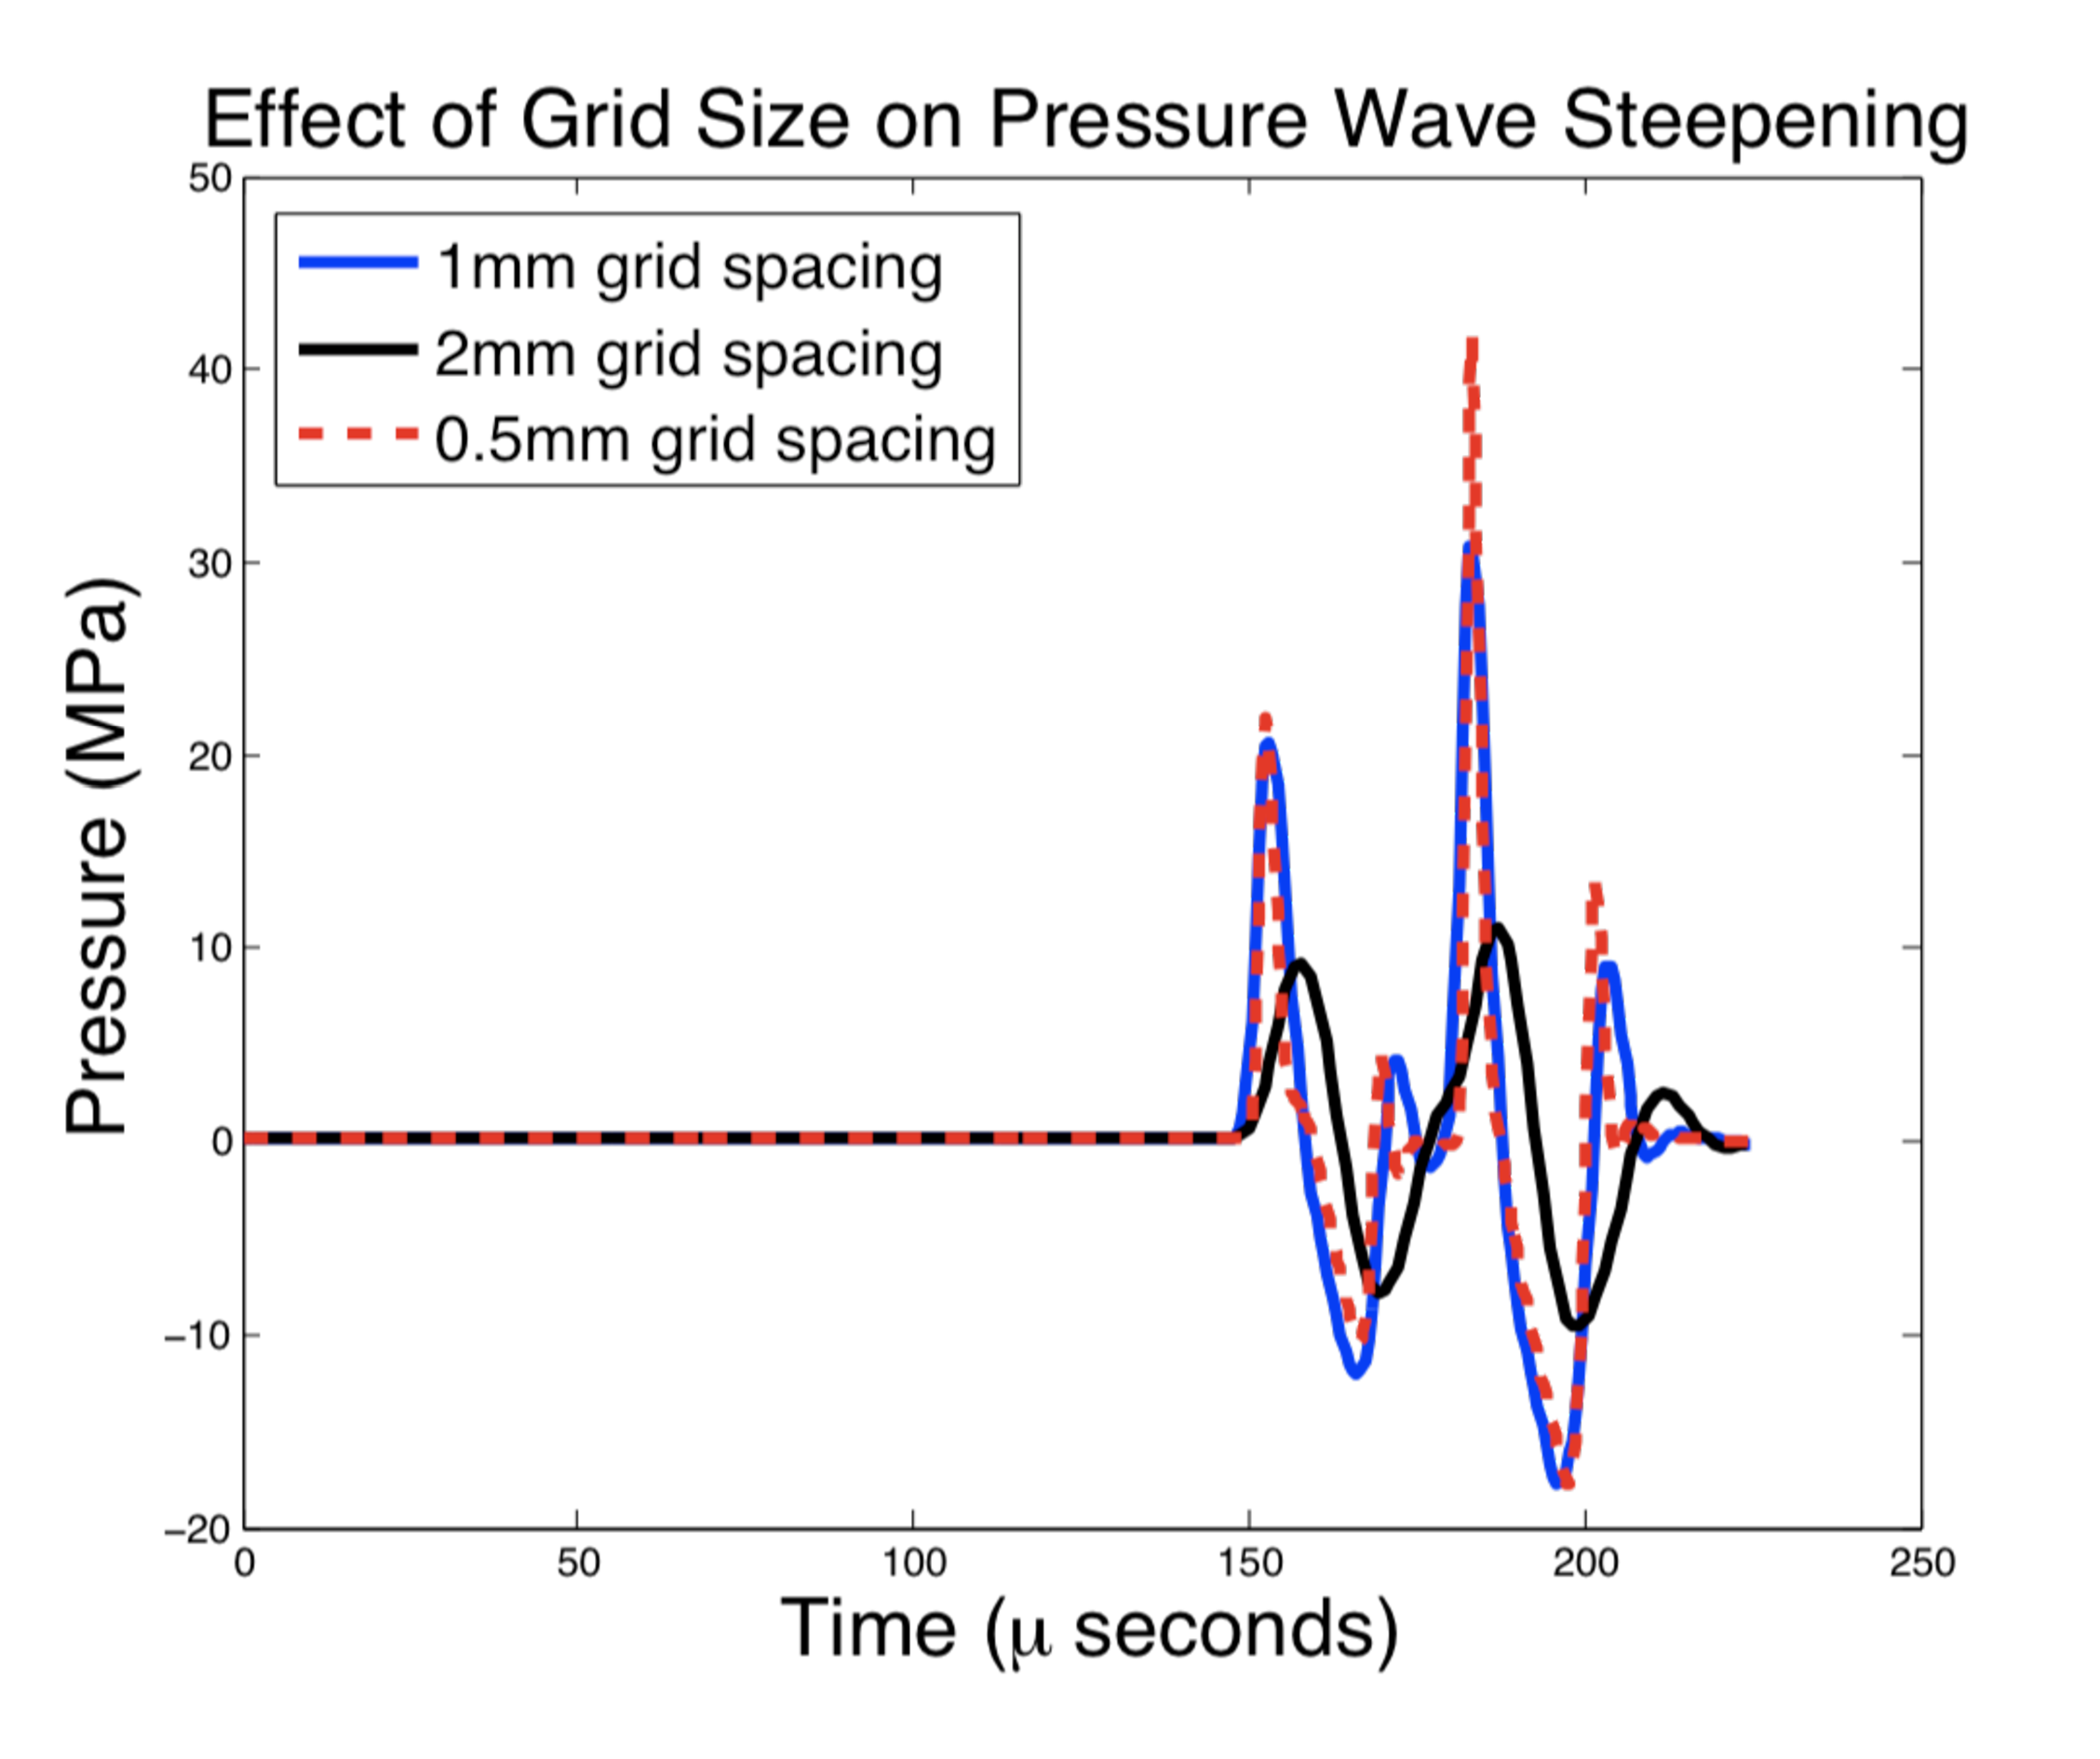
\includegraphics[height=2in, width=2in]{grid_refinement_steepening.pdf}
\label{fig:steepening}
\caption{Effect of grid size on shock wave profile}
\end{center}
\end{figure}
In order to efficiently calculate a reasonable ESWT waveform, we utilized ChomboClaw 
\cite{chomboclaw}, which uses the adaptive mesh refinement routines of CHOMBO with the wave 
propagation solvers of CLAWPACK.  This code can be run in parallel using MPI and we ran it on 
TeraGrid \cite{teragrid} system.  It has been indicated that Chombo will scale up to 10,000 processors 
\cite{collela_correspondance}.  We found that the ChomboClaw code scaled up to 128 processors, 
however we would like to do further testing on a larger system.
\begin{figure}
\begin{center}
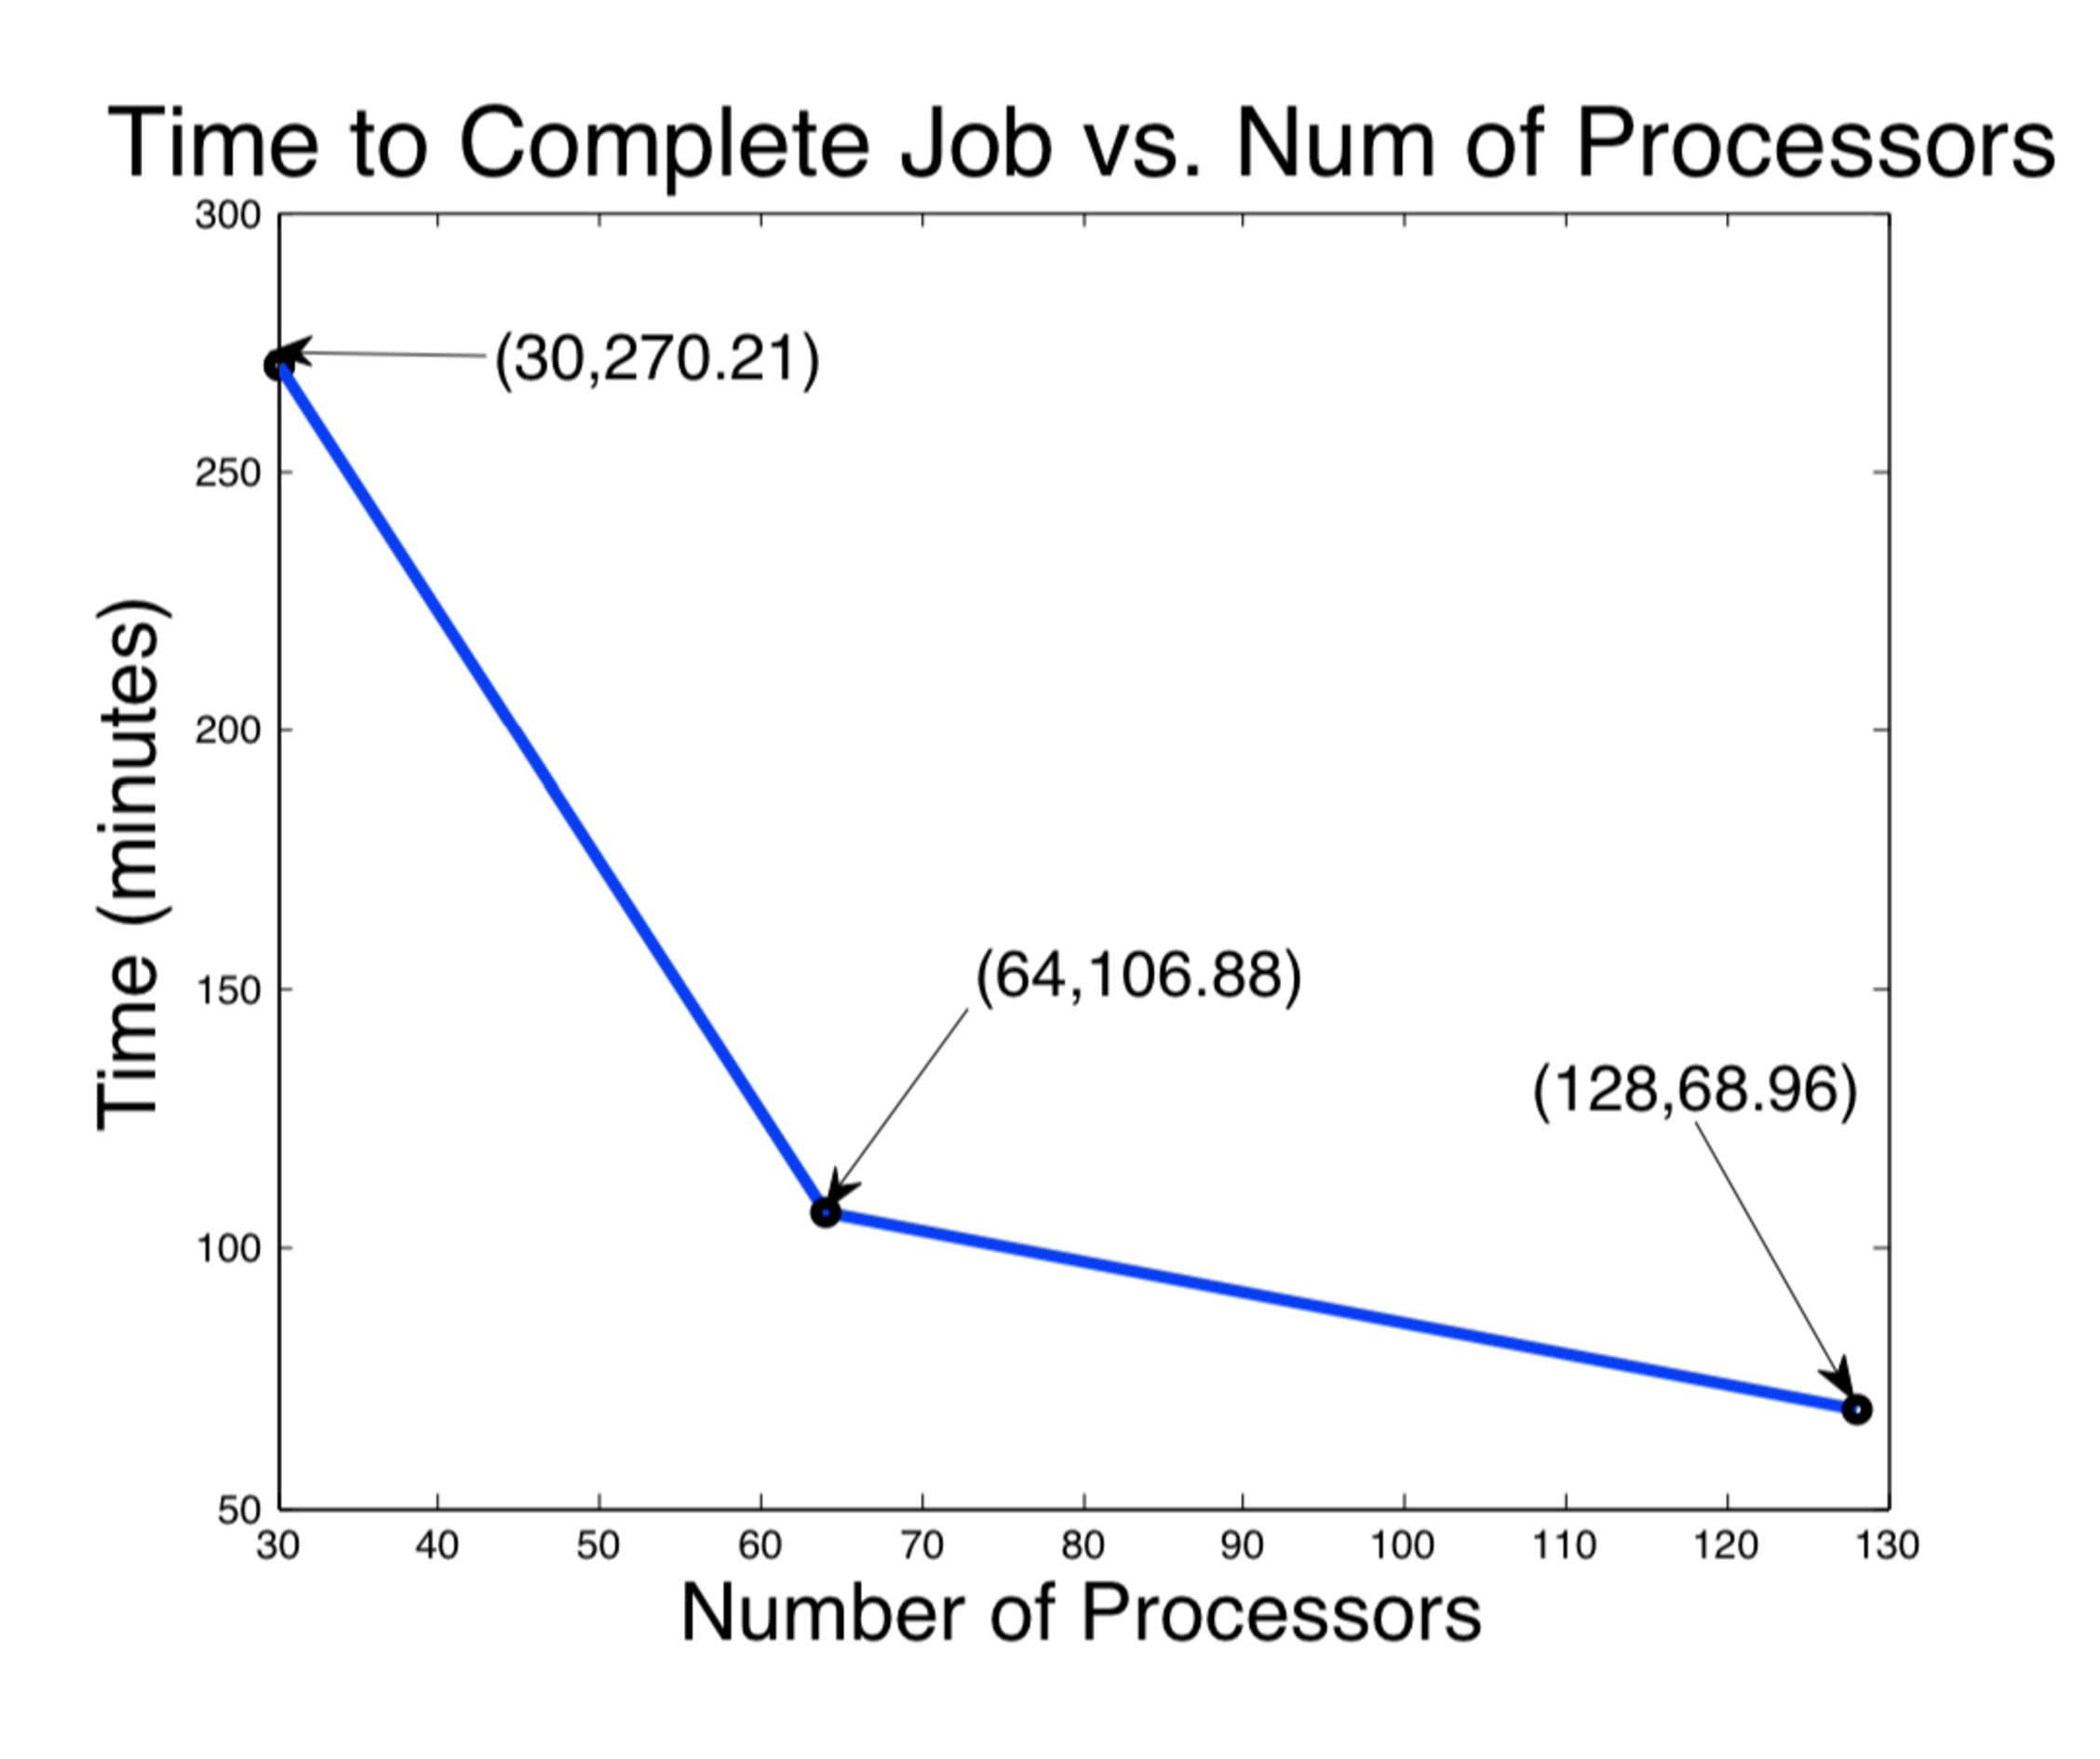
\includegraphics[height=2in, width=2in]{timing.pdf}
\label{fig:scaling}
\caption{Result from strong scaling test of ChomboClaw up to 128 processors.}
\end{center}
\end{figure}

\subsection{Interfaces and the Cartesian Grid}
\label{sec:interfaces}
Calculation series demonstrating the effective use of AMR for capturing the reflection off the curved 
ellipsoidal geometry of the lithotripter.  (Re-running this job to save better plots/pressure waveform, need 
to save the better resolution run like with the swallow tail focal region calculation.)

\begin{figure}
\begin{center}
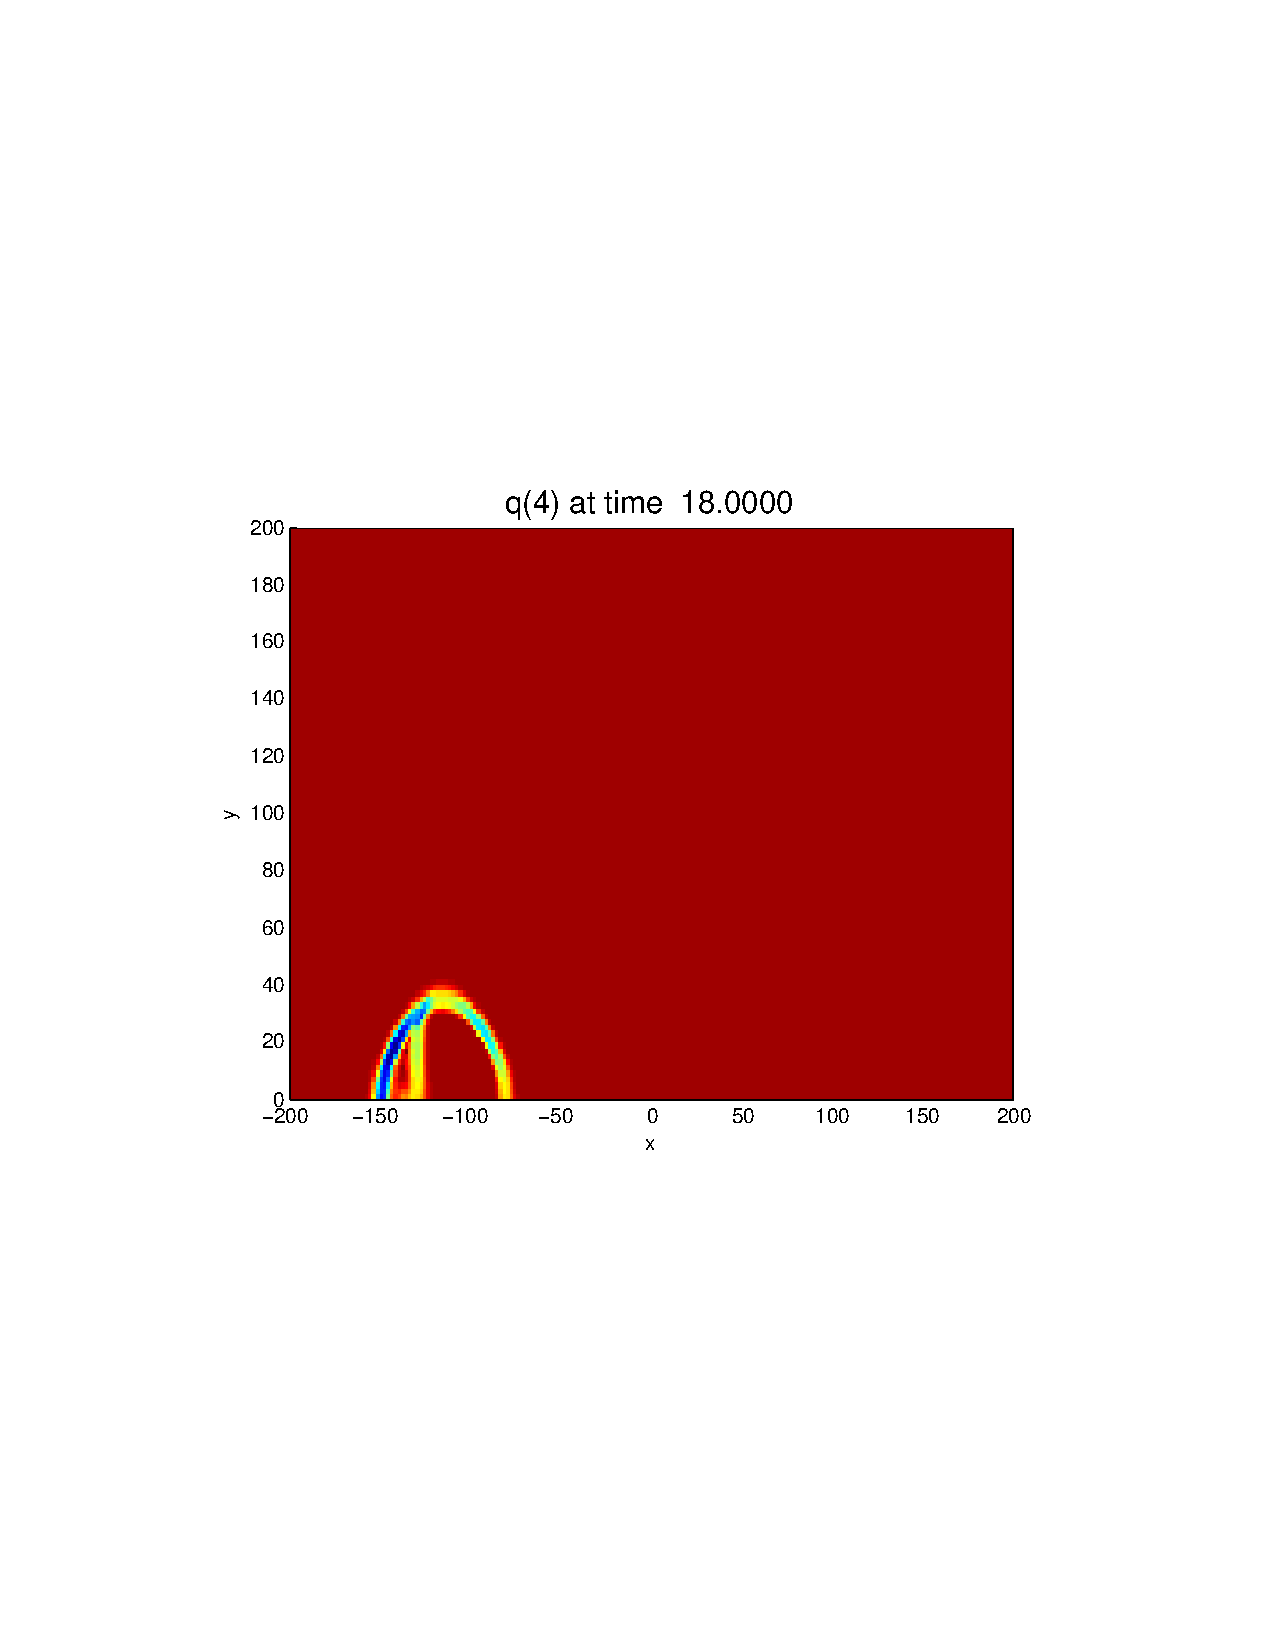
\includegraphics[height=2in,width=2in]{reflect1.pdf}
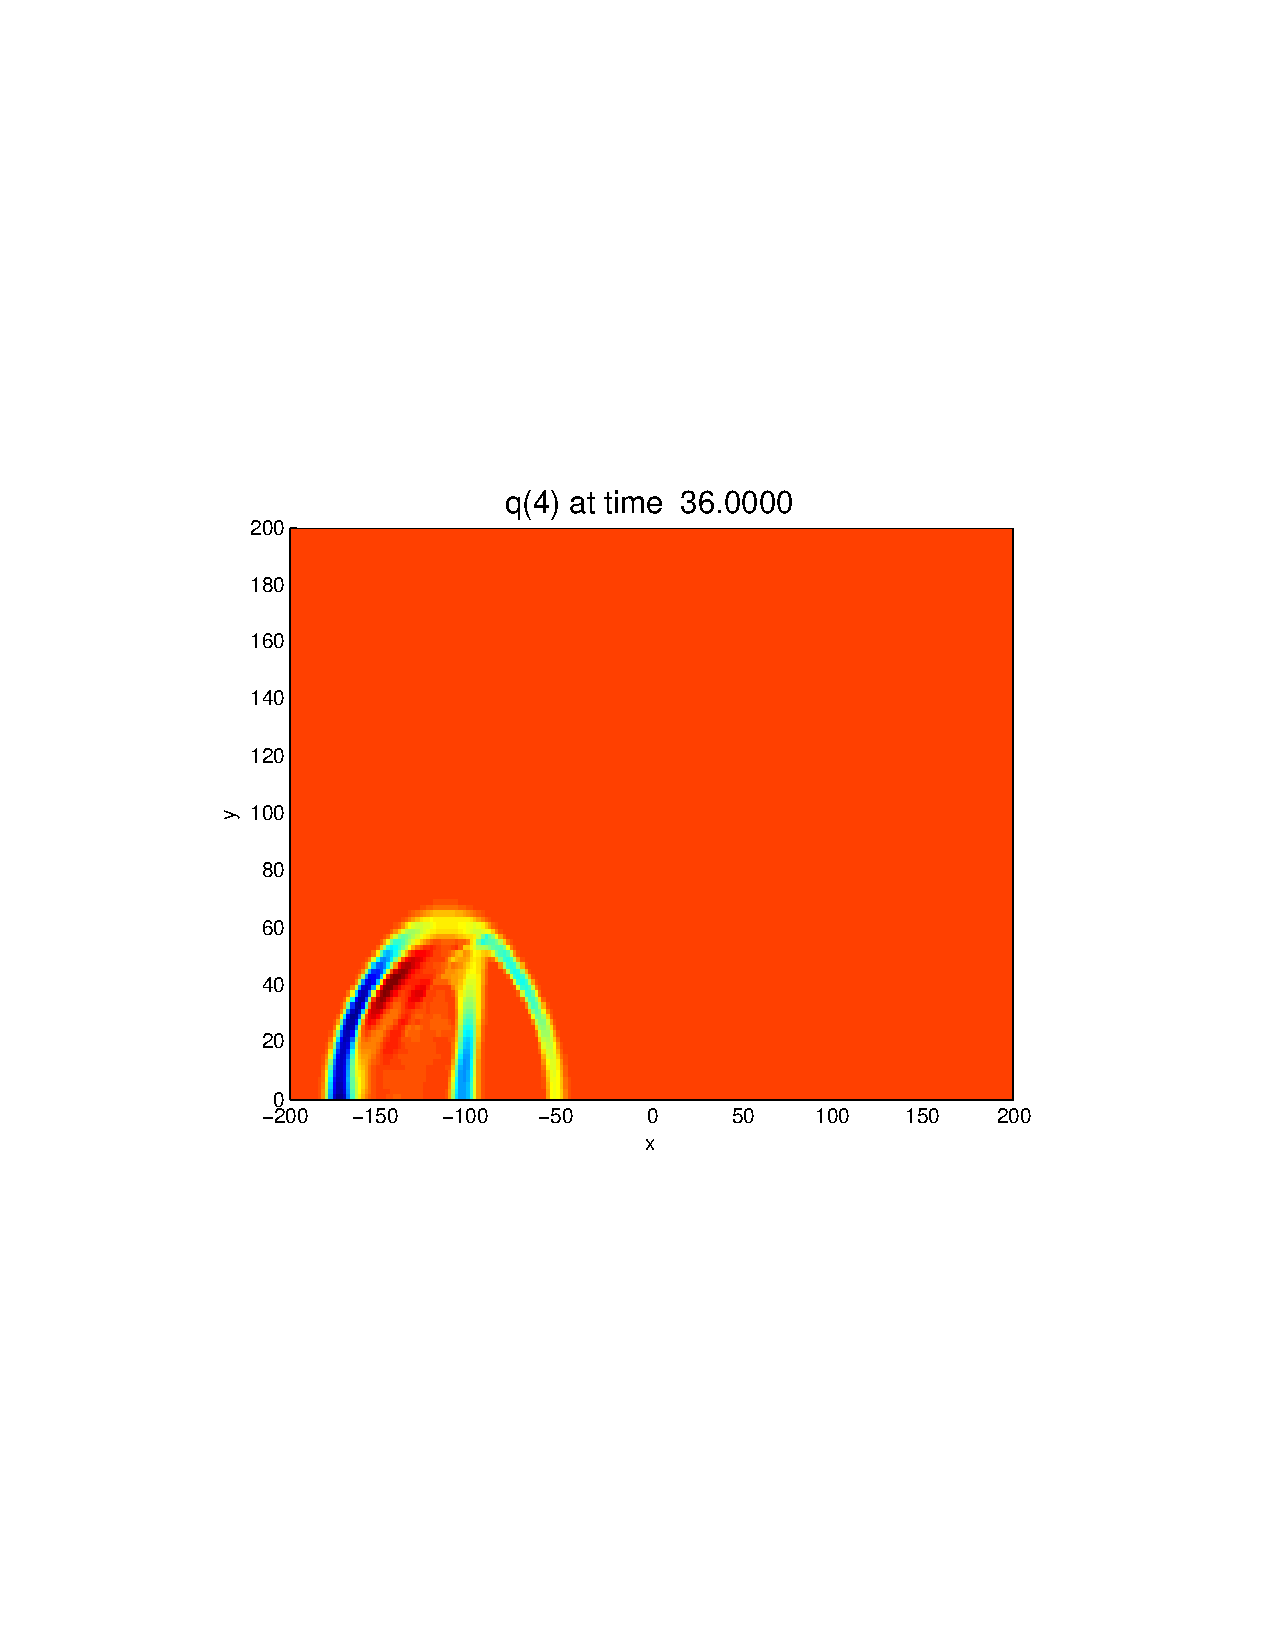
\includegraphics[height=2in,width=2in]{reflect2.pdf}
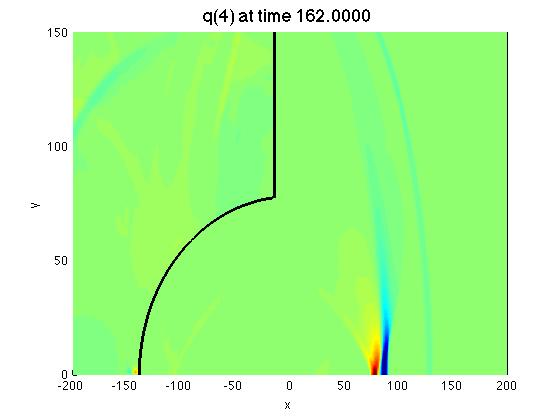
\includegraphics[height=2in,width=2in]{swallow_tail4.jpg}
\caption{Sample calculations, too coarse, will be replaced with images from a job running now}
\end{center}
\end{figure}

\begin{figure}
\begin{center}
a) 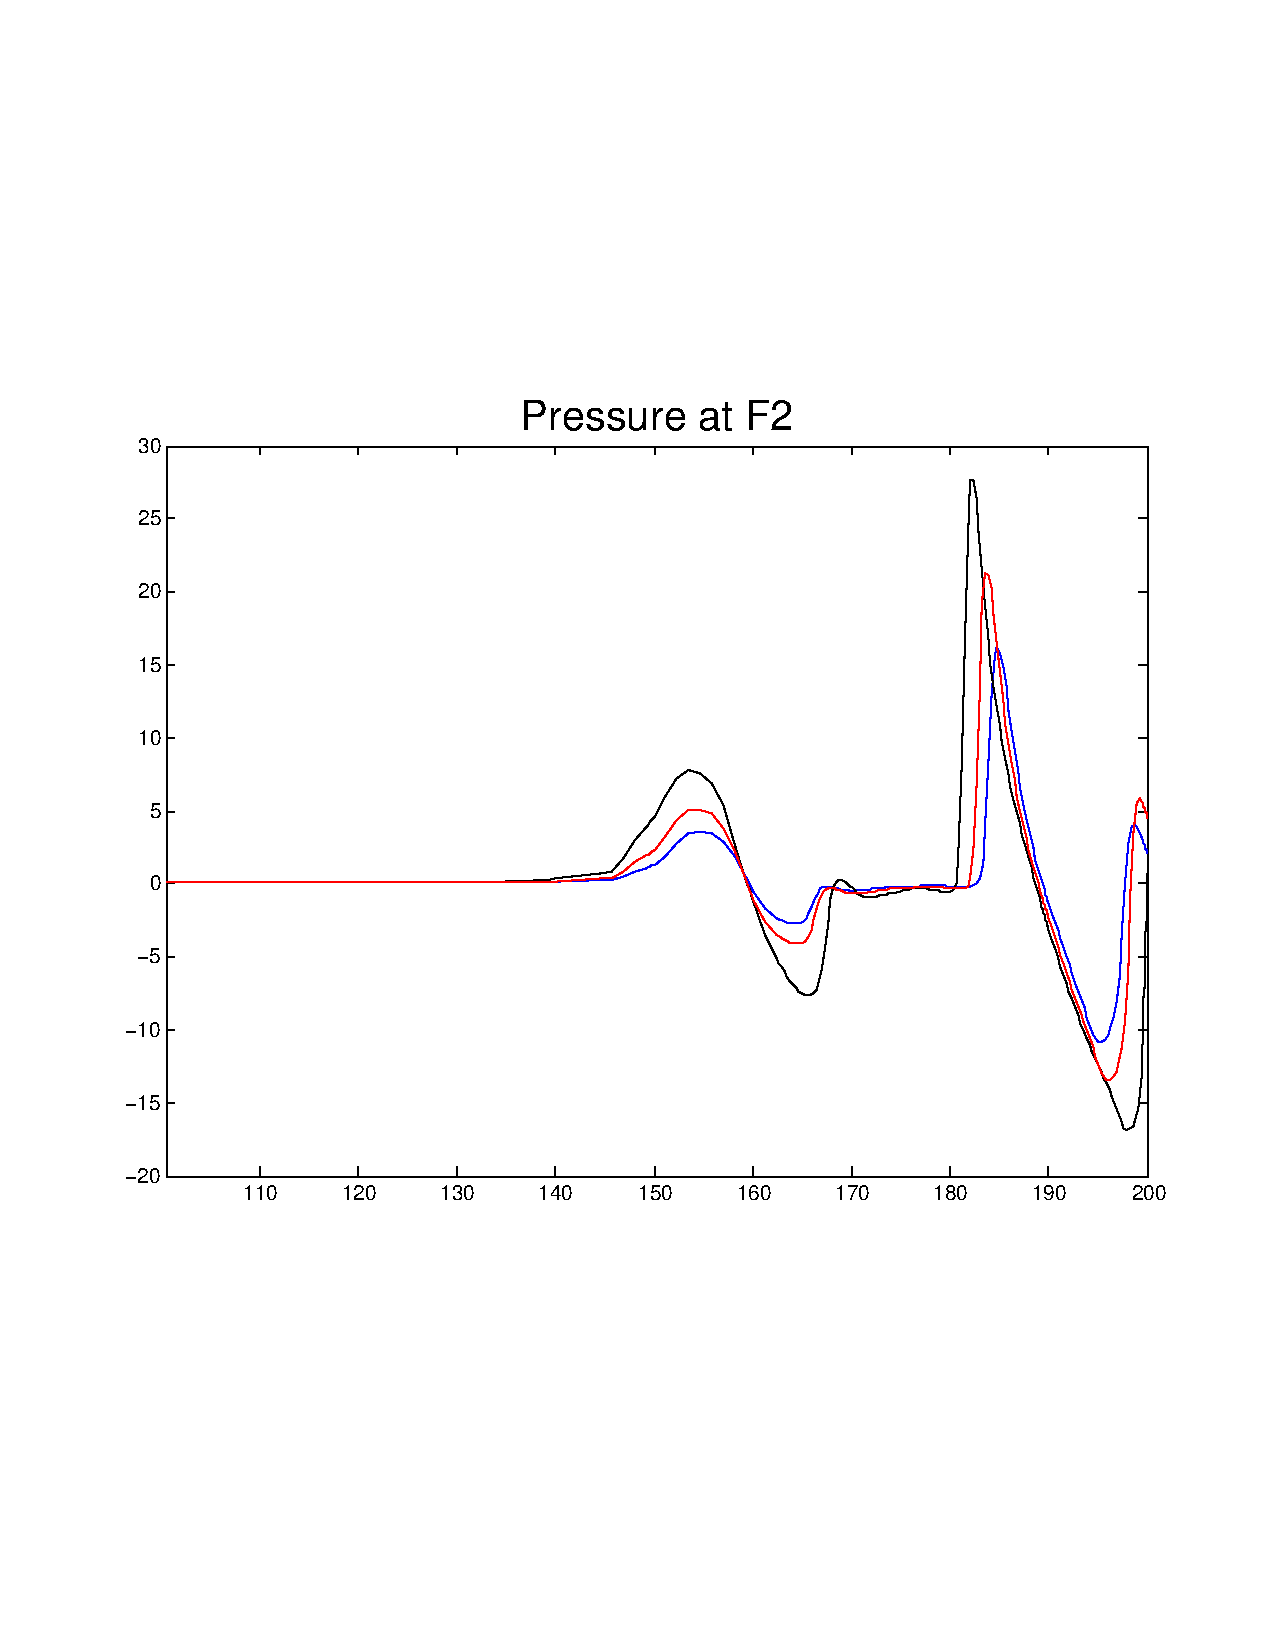
\includegraphics[height=2in,width=2in]{pressure_hm3.pdf}
b)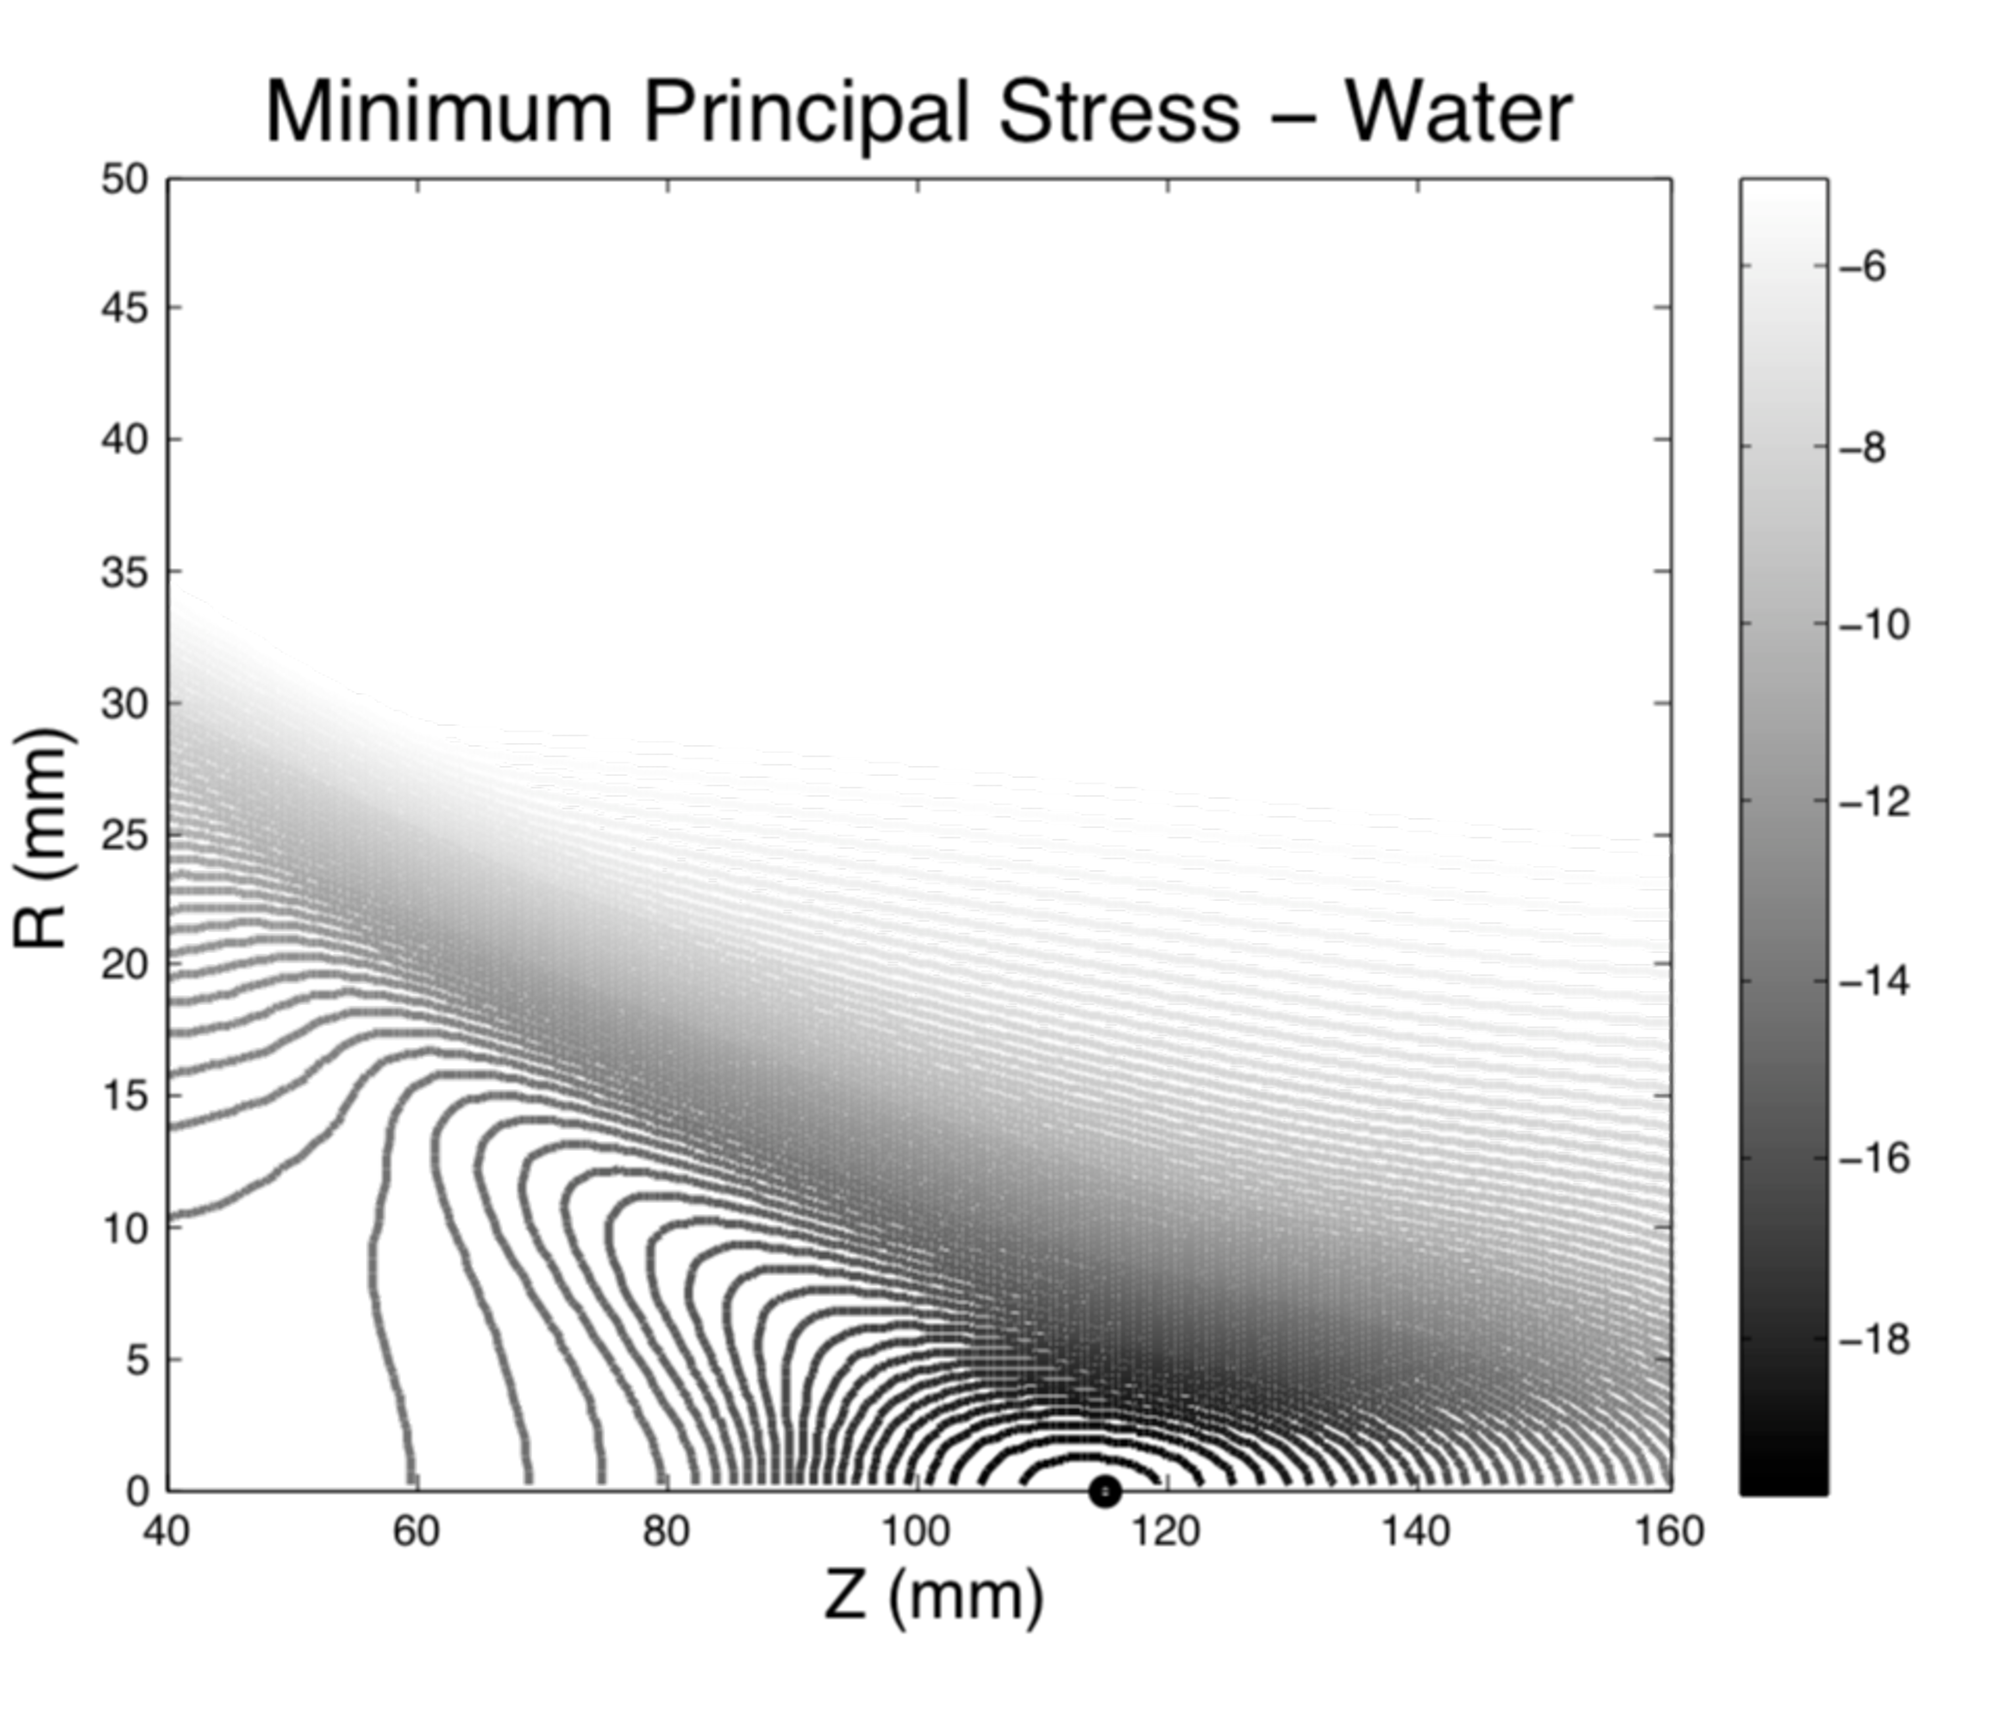
\includegraphics[height=2in, width=2in]{minimum_pstress_water.pdf}
\label{fig:scaling}
\caption{a)Redo with pressure and time-scale labels  b)Validation that our Lagrangian code generates 
the correct cigar shaped region of minimum principal stress, or maximum pressure.  This was generated 
using the 2D Axisymmetric Lagrangian code with the Tait EOS.}
\end{center}
\end{figure}

\section{Results}
\label{sec:results}
We have used this approach to model ESWT pressure waves interacting with three-dimensional bone 
geometries that we assume are comprised of idealized materials.  In some cases we model objects 
identical to those used in laboratory experiments \cite{amath_apl_nonunion}, but in others we extracted 
three-dimensional objects from CT scans of patient data \cite{fagnan_chang_ho}.  Here we present 
results that demonstrate the efficacy of the Lagrangian formulation, as well as examples of calculations 
performed using real three-dimensional geometries. 

\subsection{Heterotopic Ossification}
\label{sec:ho}
This experiment shows a calculation involving a heterotopic ossification, or a growth of bone-like 
material in soft tissue that is inhibiting the movement of the hip joint.  The composition and material 
properties of the ossification are not well understood.  We are able to use our model to investigate the 
effect of varying the material properties of the ossification as well as the strength of adhesion to the hip 
bone.  We found that the strength of the adhesion had a significant effect on the location of maximum 
stress in the object \cite{kfagnan_mchang_ho}.  Here we present a snapshot of the maximum shear and 
compressive stress calculated in the ossification. 
\begin{figure}[ht]
\begin{center}
a)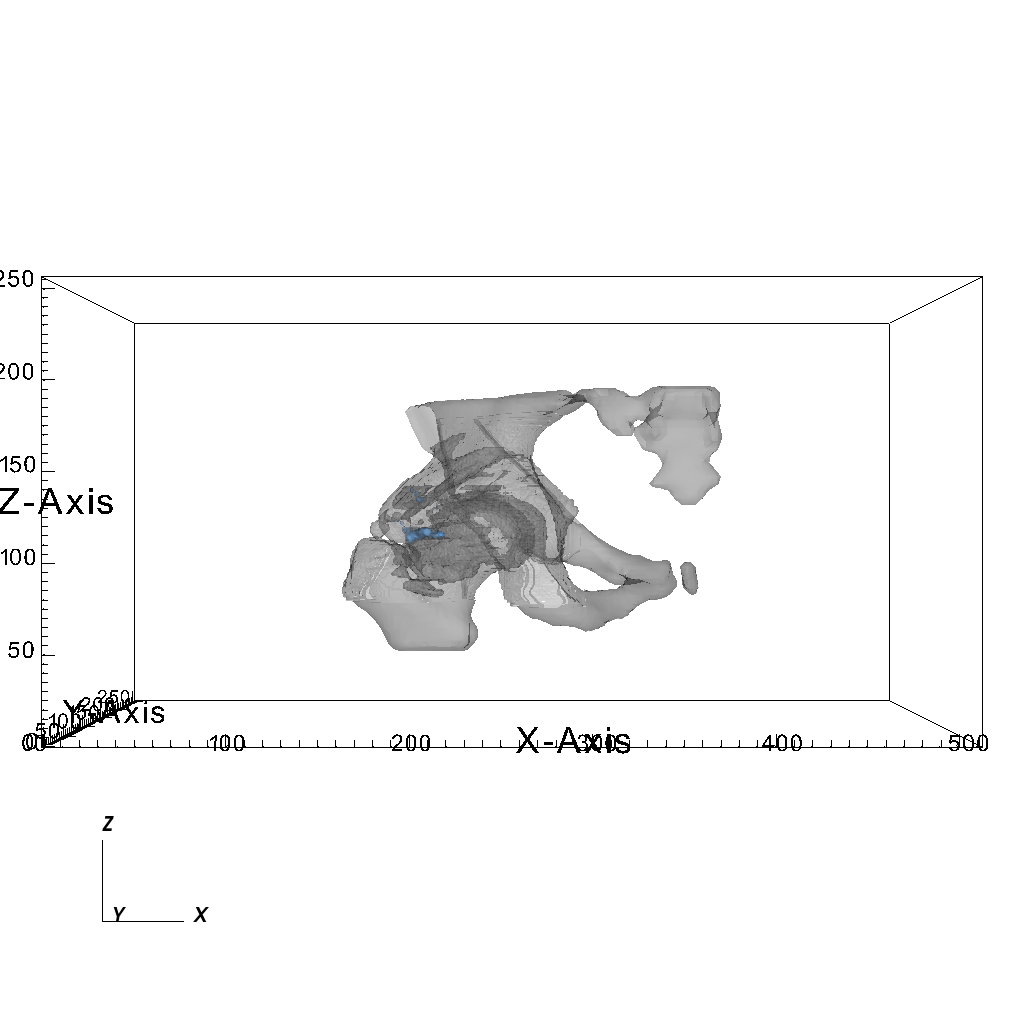
\includegraphics[scale=.25]{hip_comp_direct.png}
b)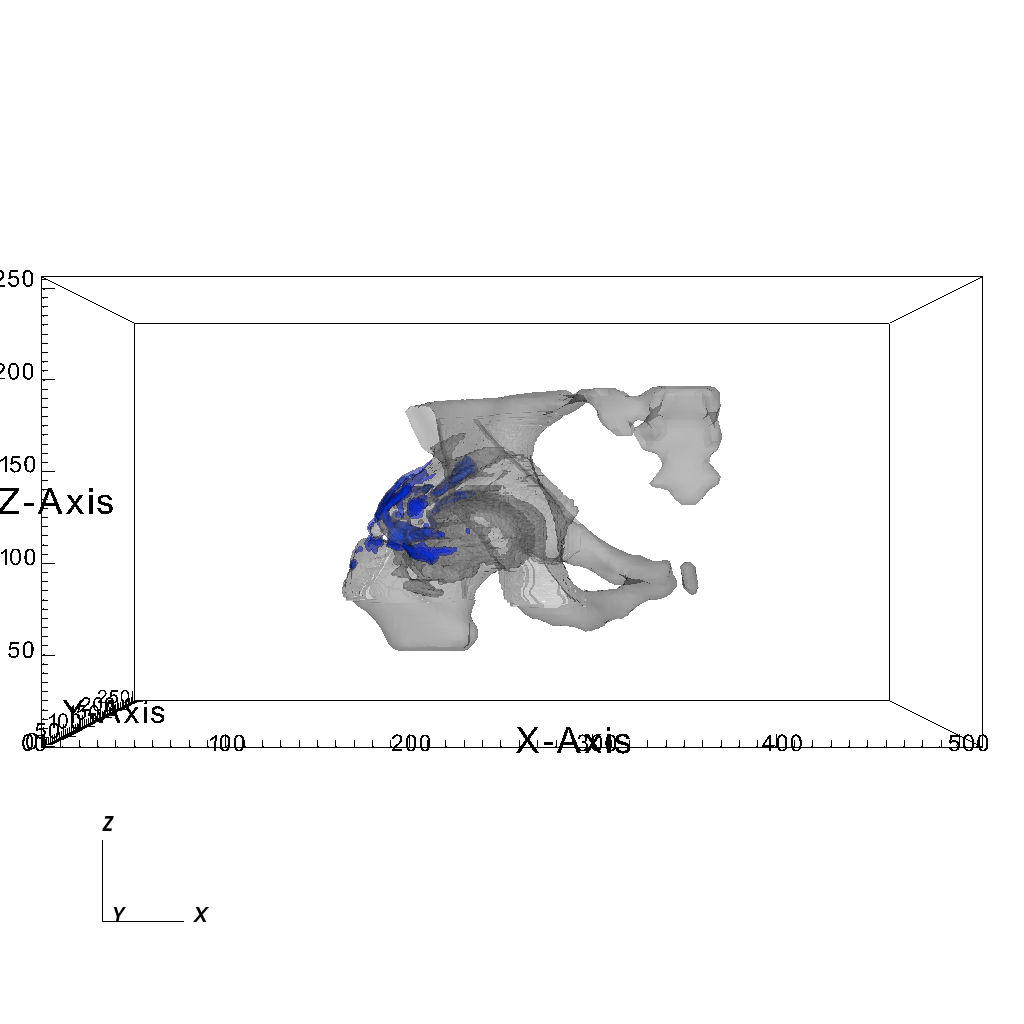
\includegraphics[scale=.25]{hip_tens_direct_ydir.png}
\caption{Isosurface of a) Maximum Compression and b) Maximum Tension in the HO shot directly.}
\end{center}
\end{figure}
(These will be a 3D embedded object, once I have figured out how to plot the stresses on the same 
figure and have the shading be different - I haven't yet determined how to do that)

\section*{Acknowledgements}
This work was supported in part by . The authors would like to thank Donna Calhoun and the ANAG 
group for their assistance with the ChomboClaw calculations.

\end{document}
